\documentclass[conference]{IEEEtran}
\IEEEoverridecommandlockouts
% The preceding line is only needed to identify funding in the first footnote. If that is unneeded, please comment it out.
\usepackage{cite}
\usepackage{amsmath,amssymb,amsfonts}
\usepackage{algorithmic}
\usepackage{graphicx}
\usepackage{textcomp}
\usepackage{xcolor}
\usepackage{multirow}
\usepackage{makecell}
\usepackage{adjustbox}
\def\BibTeX{{\rm B\kern-.05em{\sc i\kern-.025em b}\kern-.08em
    T\kern-.1667em\lower.7ex\hbox{E}\kern-.125emX}}
\begin{document}

\title{TIME SERIES ANALYSIS FOR REAL ESTATE STOCK PRICE PREDICTION USING ML/DL ALGORITHMS METHODS
}
\newcommand{\linebreakand}{%
  \end{@IEEEauthorhalign}
  \hfill\mbox{}\par
  \mbox{}\hfill\begin{@IEEEauthorhalign}
}

\author{\IEEEauthorblockN{1\textsuperscript{st} Ngo Thuy Yen Nhi}
\IEEEauthorblockA{\textit{Team 4 - IS403.O21} \\
Ho Chi Minh City, Viet Nam \\
e-mail: 21521230@gm.uit.edu.vn}
\and
\IEEEauthorblockN{2\textsuperscript{nd} Nguyen Duong}
\IEEEauthorblockA{\textit{Team 4 - IS403.O21} \\
Ho Chi Minh City, Viet Nam \\
e-mail: 21521990@gm.uit.edu.vn}
\and
\IEEEauthorblockN{3\textsuperscript{rd} Pham Duy Khanh}
\IEEEauthorblockA{\textit{Team 4 - IS403.O21} \\
Ho Chi Minh City, Viet Nam \\
e-mail: 21522211@gm.uit.edu.vn}
\and
\linebreakand
    \IEEEauthorblockN{4\textsuperscript{th} Nguyen Ngoc Ha My}
    \IEEEauthorblockA{\textit{Team 4 - IS403.O21} \\
    Ho Chi Minh City, Viet Nam \\
    e-mail: 21522351@gm.uit.edu.vn}
\and
    \IEEEauthorblockN{5\textsuperscript{th} Le Thuan Hieu}
    \IEEEauthorblockA{\textit{Team 4 - IS403.O21} \\
    Ho Chi Minh City, Viet Nam \\
    e-mail: 21522072@gm.uit.edu.vn}
}
\maketitle

\begin{abstract}
Machine learning and deep learning techniques is renowned for playing a pivotal role in the realm of Business Analytics nowadays by leveraging time-series datasets with the aspiration to provide businesses with analytics-driven insights that assist in facilitating decision-making, improve performance, and optimize processes. Due to the rapid and diverse development of algorithms, there aries a critical need to scrutinize the efficacy of them within specific domains. This paper addresses this imperative by utilizing and evaluating five distinct algorithms - FEDformer, TBATS, AR-MOS, Kalman Filter, and ResNet towards three different time-series datasets from three distinguished real estate companies in Viet Nam. Within the context of this study, the objective is to analyze and forecast the trajectory their stock prices based on their historical daily stock price records. The study delves into an extensive comparative analysis of these algorithms' capabilities and outlines a detailed methodology that illuminates the intricacies of each algorithm's application and the rationale behind their selection. Subsequently, the study applies the findings obtained from the completed analyses to elucidate the strengths and limitations of each approach. Ultimately, through systematic rigorous evaluation and comparison, this paper aims to enhance the understanding of the suitability and competently of these algorithms for stock prices analysis and prediction within the real estate domain in Viet Nam.\\
\end{abstract}

\begin{IEEEkeywords}
Analytic, ETS, Comparison, Efficacy, FEDformer, Kalman Filter, Market capitalization, Prediction, Real estate, ResNet, Stock prices, TBATS, Time-series.
\end{IEEEkeywords}

\section{\textbf{Introduction}}
In the contemporary era shaped by rapid societal and technological advancements, a typical modern business or industrial organization is constantly in demand of a cutting-edge and robust analytical tools for effective decision-making and risk management. Therefore, there arises a pressing need for advanced analytical tools and methodologies to navigate and extract insights from vast volumes of data.\\ 
In general, the world, and specifically Viet Nam, the real estate sector has experienced rapid growth and transformation in recent years, driven by urbanization, economic development, and foreign investment. Amidst this dynamic landscape, accurate estate analysis and forecasting play a pivotal role in facilitating informed decision-making and strategic planning for real estate companies. Stock prices, as a key indicator of a company's value and performance, serves as a crucial metric for investors, analysts, and industry stakeholders alike. Accurate prediction of market capitalization not only aids investors in decisions making but also assists real estate companies in strategizing their operations and investments effectively. \\
Given the importance need for robust analysis and predictive models within the real estate domain in Viet Nam, Machine learning and Deep learning techniques have emerged as powerful tools in this regard, offering the potential to uncover patterns, trends, and predictive signals within time-series datasets. Against this backdrop, this study investigates the capabilities of various machine learning and deep learning algorithms in analyzing and forecasting stock prices for three prominent real estate companies in Vietnam (DXG, DIG and NVL). Ultimately, the objective is to elucidate the efficacy and comparative performance between the five methodologies of ML/DL algorithms - FEDformer, TBATS, AR-MOS, Kalman Filter, and ResNet by leveraging three different time-series datasets based on historical daily stock price records of those three Vietnamese prominent real estate companies. \\
The primary goal of this paper is twofold as it embarks on a comprehensive examination of the five algorithms methodologies: \\
Firstly, to evaluate the performance and effectiveness of the five selected algorithms in analyzing and forecasting daily stock price data for the specified real estate companies.
Secondly, to conduct a comparative analysis of their efficacy and performance, highlighting the strengths as well as limitations of each approach, and examine the suitability and competency of these algorithms in the context of real estate market analysis. \\
The structure of this paper is organized to provide a comprehensive understanding of these objectives to outline the suitability and competency of these algorithms. Following this introduction, the subsequent section – Related Work, reviews existing literature, journals and research relevant to ML/DL applications in real estate analysis. Then, the Material section provides the dataset descriptions, data selection criteria, and descriptive statistics employed in this study. Subsequently, in the Methodology section, the study presents the criteria for algorithm selection, and the evaluation metrics utilized in this investigation. In the following section, the Results section presents the findings derived from the application of each algorithm and the evaluation methods deployed. Finally, the Conclusion section summarizes the key findings, discusses their implications, and outlines avenues for future considerations. 

\section{\textbf{Related Works}}

% Openning
Stock prices can be influenced due to various factors such as company’s status, market sentiment, or economic indicators, etc. In recent years, a plethora of studies had been dedicated for analysing and predicting stock prices, employing a variety of ML/DL algorithms, and statistical models. The methodologies encompass statiscal and analytical approaches achieved through a diverse selection of those ML/DL techniques and hybrid forecasting methods.\\ 
Therefore, this section focuses on critically examining existing literatures and research papers pertinent to the comparative performance of various ML/DL algorithms as well as statistical models’ applications in stock price analysis and prediction. The aim is to contextualize recent studies, identifying key trends, methodologies, and findings in the field and provide an overview of the ML/DL algorithms used in this work comparing with others in different scenarios. This will assist further the investigation and provide suggested selection of methodologies applied in the study to evaluate and determine the efficacy of each ML/DL algorithms and models utilized in this research.\\

% FEDfomer
In 2023, A. T. Haryono et al. \cite{b1} had stated in their published article titled "Transformer-Gated Recurrent Unit Method for Predicting Stock Price Based on News Sentiments and Technical Indicators" that the FEDformer architecture, another transformer of time-series, outperformed the traditional Transformer and its counterparts such as AutoFormer, Informer, and Reformer in predicting stock prices. Additionally, the performances of AutoFormer, Informer, and Reformer were also stated to be more advanced compared to ARIMA and LSTM models. For stock prices forecasting, the evaluation methods deployed including R2, RMSE, MSE, and MAPE with the time lag variants of 5, 10, 20, 100, and 200 for a specified stock issuer. The outcomes revealed that FEDformer possessed a superior efficacy with an RMSE score 83.08\% lower than Transformer and 84.83\% lower than Informer. Futhermore, the MAPE score of FEDformer was also 85.17\% lower than Transformer and lower by 96.66\% compared to Informer. Without a doubt, FEDformer emerges as a dominant selection among other transformer models in resolving limitations on trend capture in long-term time series forecasting.  \\

% ARIMA
S. Khan et al. \cite{b2} performed their study on the implementation and comparison of three different ARIMA models in Time Series Forecasting, which was published in 2020 under the title "ARIMA Model for Accurate Time Series Stocks Forecasting". They indicated that the customize ARIMA(p,D,q) model with the value of (1,1,33) produced the best result out of the other two models: Auto ARIMA(4,1,4) model and customize ARIMA(1,2,33) model. Initially, the MAPE evaluation method demonstrated little to no differences among the three models as the MAPE score for each model were 98.88\% for Auto ARIMA(4,1,4), 99.74\% for ARIMA (1,1,33) and 99.75\% for ARIMA (1,2,33). Since the forecasting accuracy of the three models displayed respectively similar values, they administrated further tests by holding out 50\% of the data and forecasting the remaining 50\% to determine the best accuracy. As a result, the customize ARIMA (1,1,33) model showed better accuracy from the addition holdout test with the ability to maintain the continuity in value. Despite being an older model, ARIMA serves as the foundation for other algorithms and remains one the most widely used models in the field of economics and finance, particularly for stock forecasting, and above all, possesses the potential to achieve accurate prediction on stock prices data. \\

% LSTM
In a 2017 published article about Time Series Forecasting with the title "LSTM Neural Network with Emotional Analysis for Prediction of Stock Price", Qun Zhuge et al. \cite{b3} implemented a study to investigate the effectiveness of LSTM and its potential as a predictive model in the realm of stock prices prediction, particularly for the data that were non-linear, long-term dependent, influenced by noises and many other factors. After executing a series of experiments, they highlighted the exceptional performance of the LSTM model compared to traditional neural network, thus improving the prediction accuracy. The result generated by the proposed model utilizing different input variables merged together (M2) produced better predictions than the model just applying a single type of input variables (M1) due to the mean MSE score of 0.000407 for M1 being greater than 0.000286 for M2. Moreover, the mean \textit{B} percentage of M2 was only 25.93\% of that of M1, further supporting the main idea of the study. In addition, this paper demonstrated the LSTM model's capability to learn the long-term dependence existing in the given stock data, there by improving the accuracy of the experiment.\\

% RNN
Selvin et al. \cite{b4} put the trajectory on identifying the latent dynamics in the given stock data utilizing Deep Learning mehthods such as RNN and LSTM. When ARIMA having been taken to the comparison, the result came up with the fact that the performance of RNN and LSTM model far surpassed than that of ARIMA model, with a mean error percentage of 29.86\%, while RNN and LSTM only reached roughly 5.21\% on three different datasets. Besides, RNN's mean error percentage was 5.12\%, which is slightly smaller than that of LSTM for 5.31\%. Although LSTM and RNN architecture cannot capture the dynamical changes accurately due to the inconsistency of the patterns and dynamics within the stock market system, they have proven to be capable of capturing hidden dynamics and enhancing precision for predictive purposes.\\

% GRU
C. Qi et al. \cite{b5} addressed a problem about the stock price data being non-linear and frequently causing stochastic deterioration as well as time lag in prediction results, there by, leading to the existence of neural networks underperforming for predictive purposes. To solve this problem, they applied the GRU model and the GRU based CEEMDAN–wavelet model which showed the successfully enhanced accuracy and the subsided the time lag issues. This was evidenced by the RMSE evaluation scores achieved that the GRU and based CEEMDAN–wavelet model scored 17.07 and 12.99, respectively, outperformed the ARIMA and ANN model that possessed the score of 49.376 and 22.47. After verifying various evaluation indicators, the paper demonstrated that the applied models were proper and superior substitutes for traditional models in terms of stock prices predictions.\\

% ETS
Another study conducted in 2020 by Zhanao et al. \cite{b6} issued an efficacy comparison between ETS and ARIMA models in predicting stock prices and presenting viable and general approaches to be able to improve the understanding of stock price prediction for individual stock. The research found that the ARIMA model was a better fit than ETS, with its variant ARIMA(2,1,3) serving as best possible model for the time range and data exploited in the study. This was verified by the slightly smaller error values that ARIMA models had comparing to those observed from ETS model, with an RMSE of 0.409 for ETS while for the ARIMA(2,1,3) was 0.408. Ultimately, this study works best as a guide for potential investors with a demand for short-term predictions. \\

% ResNet
In a study conducted by B. Song et al. \cite{b7} in 2018 titled “Stock Price Trend Prediction Model Based on Deep Residual Network and Stock Price Graph”, ResNet model was introduced for stock prices prediction and exhibited the average accuracy of 0.40, which surpassed the stochastic indicator of 0.33 when using the stock price graph as input. The paper compared the ResNet model with three selected widely used financial time-series prediction models: SVM, DNN, and CNN. Overall, ResNet and CNN variants demonstrated the highest accuracy and showcased the most stablility in the classifier evaluation index. The deep learning models, such as ResNet, CNN, and DNN, were found to be superior to SVM due to their ability to capture the hidden dynamics of stocks with their complex network structure. Additionally, CNN and ResNet filter features through convolution operations, optimize the learning process, and mitigate overfitting compared to DNN, thereby improving accuracy. \\

%LR, TBATS, Kalman Filter
In terms of machine learning techniques, R. Seethalakshmi \cite{b8} uses linear regression to identify which attributes significantly affect the closing value of stocks. They concluded that features including open, high, low, volume, and adjusted close were fitted with an R² value of 0.997, indicating that these features are essential for accurately predicting the closing value. I. Sadia et al. \cite{b9} applied TBATS, known for its robustness in time series forecasting, was employed to effectively capture the complex dynamics of stock price movements. This approach is achieved the minimum convergence time of 4.9835 seconds and the figure of 2.823 in MAPE, demonstrating its efficiency in handling large-scale financial data and real-time cryptocurrency price movements. 

N. Deepika et al. \cite{b10} improve the quality of stock predictions via implementing a Kalman filter to remove noise from extracting relevant indices from stock data. Their results are promising. The proposed method, which combines an attention-gated LSTM (AG-LSTM) with a Kalman filter, achieved significantly better performance compared to a standard LSTM model without the filter. The comparison of MSE for Apple Company stock prediction revealed a significant difference: 0.0514 with the Kalman filter and 0.2451 without it. This substantial reduction in MSE suggests that incorporating a Kalman filter can enhance the accuracy of stock price predictions.


% Closing
Collectively, these studies contribute to the increasing collection of literature on ML/DL applications in real estate stock price prediction, exhibiting the versatility and effectiveness of various models across different market conditions and time frames. By synthesizing key findings and methodologies, this section provides a comprehensive overview of the state-of-the-art techniques and avenues for future research in the field.

\section{\textbf{Materials}}
\subsection{Dataset}\label{AA}
In this article, we scrutinize the stock prices data of three following prominent real estate companies in Viet Nam:
\begin{itemize}
    \item Dat Xanh Group (DXG), 
    \item Development Investment Construction JSC (DIG),
    \item No Va Land Investment Group Corporation (NVL).
\end{itemize}
Each dataset presents a record of each company's stock prices, thoroughly documented spanning from January 1, 2018, to March 22, 2024, with a daily time frame on trading activities. These datasets are sourced from Investing.com, a reputable financial platform renowned for providing comprehensive trading information for companies or financial organization.\\
The datasets feature the following array of variables, providing crucial insights and materials for the study. The variables include:
\begin{itemize}
    \item Date: Presenting the trading date in the format DD/MM/YYYY.
    \item Price: Denoting the closing price of the stock on the respective trading day.
    \item Open: Signifying the opening price of the stock on the respective trading day.
    \item High: Presenting the highest recorded of the stock price within the trading day.
    \item Low: Indicating the lowest recorded of the stock price during the trading period.
    \item Vol: Evaluating the trading volume for each day, represented by the number of shares traded (expressed in millions of shares).
    \item Change (\%): Determining the percentage change in the stock's value compared to the preceding trading day.
\end{itemize}
All data referring to stock-related metrics are denominated in Vietnamese Dong (VND), ensuring consistency and coherence throughout the analysis.

\subsection{Descriptive Statistics}

\begin{figure}[htbp]
\centering
    \begin{minipage}{0.23\textwidth}
    \centering
    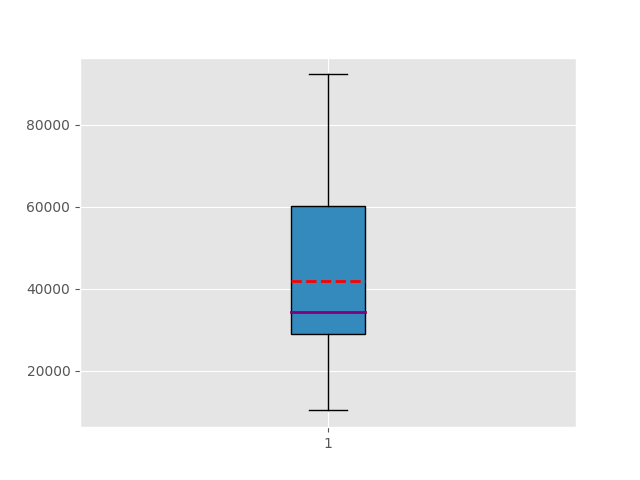
\includegraphics[width=1\textwidth]{Boxplot_NVL.png}
    \caption{NVL stock price's boxplot}
    \label{fig:nvl_boxplot}
    \end{minipage}
    \hfill
    \begin{minipage}{0.23\textwidth}
    \centering
    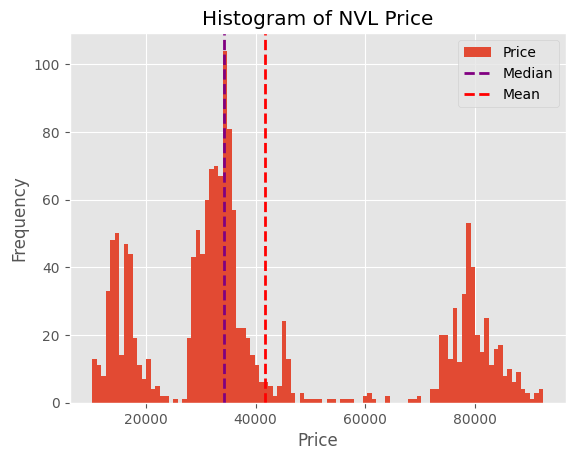
\includegraphics[width=1\textwidth]{Histogram NVL.png}
    \caption{NVL stock price's histogram}
    \label{fig:nvl_histogram}
    \end{minipage}

    \vspace{0.5cm} % Add vertical space between the sets of figures

    \begin{minipage}{0.23\textwidth}
    \centering
    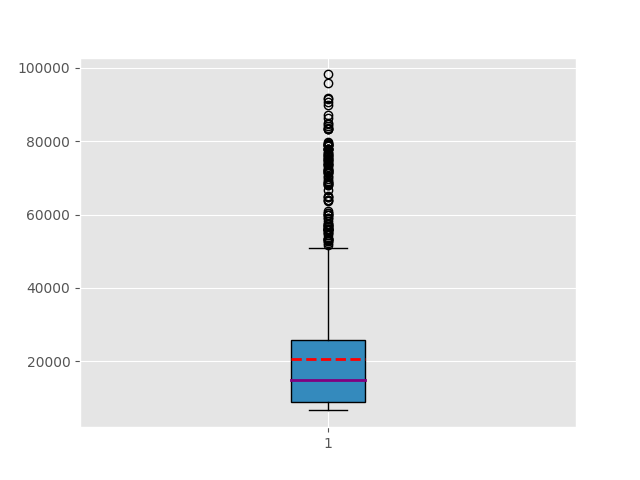
\includegraphics[width=1\textwidth]{Boxplot_DIG.png}
    \caption{DIG stock price's boxplot}
    \label{fig:dig_boxplot}
    \end{minipage}
    \hfill
    \begin{minipage}{0.23\textwidth}
    \centering
    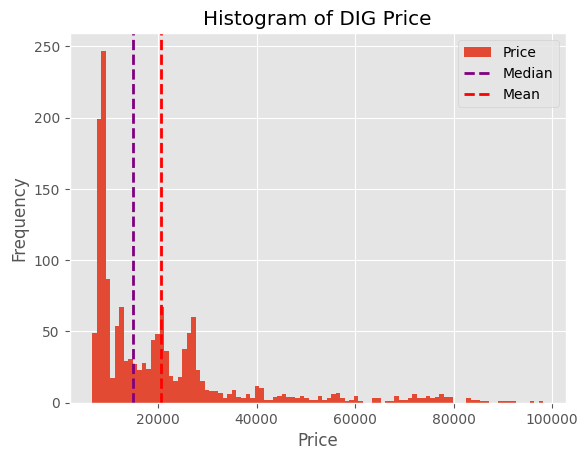
\includegraphics[width=1\textwidth]{Histogram DIG.png}
    \caption{DIG stock price's histogram}
    \label{fig:dig_histogram}
    \end{minipage}

    \vspace{0.5cm} % Add vertical space between the sets of figures

    \begin{minipage}{0.23\textwidth}
    \centering
    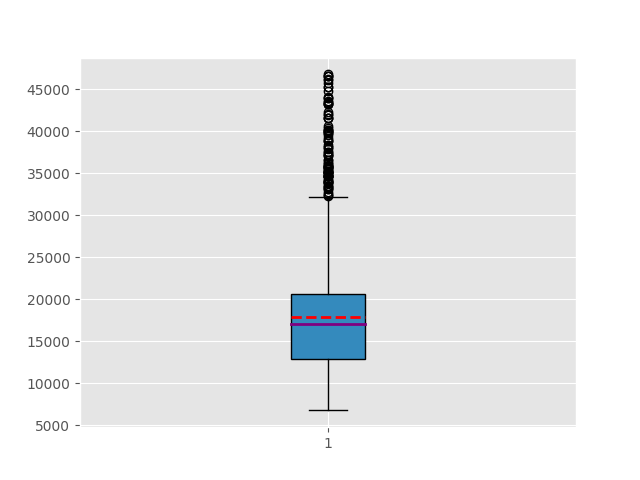
\includegraphics[width=1\textwidth]{Boxplot_DXG.png}
    \caption{DXG stock price's boxplot}
    \label{fig:dxg_boxplot}
    \end{minipage}
    \hfill
    \begin{minipage}{0.23\textwidth}
    \centering
    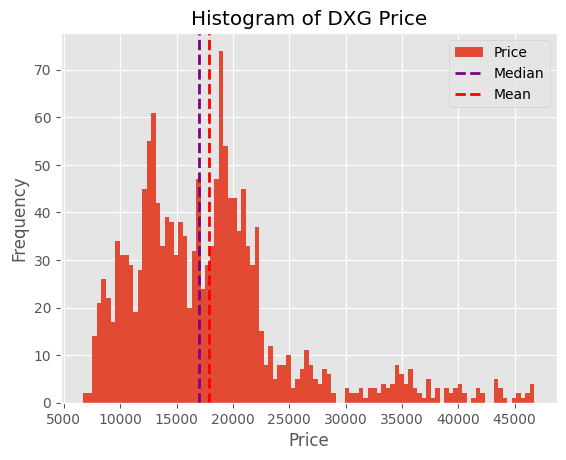
\includegraphics[width=1\textwidth]{Histogram DXG.png}
    \caption{DXG stock price's histogram}
    \label{fig:dxg_histogram}
    \end{minipage}
\end{figure}

\begin{table}[htbp]
\caption{DXG, DIG, NVL’s Descriptive Statistics}
\begin{center}
\begin{tabular}{|c|c|c|c|}
\hline
\textbf{Descriptive}&\multicolumn{3}{|c|}{\textbf{Company}} \\
\cline{2-4} 
\textbf{Statistic} & \textbf{\textit{DIG}}& \textbf{\textit{DXG}}& \textbf{\textit{NVL}} \\
\hline
Count & 1552 & 1552 & 1552  \\
\hline
Mean & 20575.539 & 17846.990 & 41771.515\\
\hline
Std & 16677.794 & 7144.933 & 23474.855\\
\hline
Min & 6591.800 & 6739.100 & 10250\\
\hline
25\% & 8852.700 & 12814.250 & 28928\\
\hline
50\% & 14799.700 & 17000 & 34248\\
\hline
75\% & 25800 & 20586.350 & 60244.250\\
\hline
Max & 98196.700 & 46750 & 92366\\
\hline
\end{tabular}
\label{tab1}
\end{center}
\end{table}

\newpage
\section{Methodology}
\subsection{Linear Regression}
Linear regression is a linear approach for modeling the relationship between a scalar response and one or more explanatory variables. In linear regression, the relationships are modeled using linear predictor functions whose unknown model parameters are estimated from the data which are called linear models. Linear regression model follows a very particular form, a regression model is linear when all terms in the model have a constant or a parameter multiplied by an independent variable. And by adding the terms together, the equation is formed:
\[ Y = \beta_0 + \beta_1 X_1 + \beta_2 X_2 + \ldots + \beta_p X_p + \epsilon \]
Where:
\begin{itemize}
    \item $Y$: dependent variable (affected by other variables)
    \item $X_1, X_2, X_p$: independent variables (affecting other variables)
    \item $\beta_0$: regression constant (or intercept). This is the index indicating the value of $Y$ when all $X$ are 0 (no $X$). When represented on the XY graph, $\beta_0$ is the point on the $Oy$ axis where the regression line intersects.
    \item $\beta_1, \beta_2, \beta_p$: regression coefficients, also known as slope coefficients. This index indicates the level of change in $Y$ caused by the corresponding $X$.
    \item $\epsilon$: error term. This index, the larger it is, makes the prediction accuracy of the regression less accurate or more deviated from reality.
\end{itemize}

\subsection{ARIMA}

ARIMA stands for Autoregressive Integrated Moving Average. The ARIMA model is based on the Box and Jenkins method of using three different concepts: autoregressive (AR) model, moving average (MA) model, and integration, together classified as an ARIMA $(p, d, q)$. It is a quantitative forecasting model over time, where the future value of the predictor variable will depend on the movement trend of that object in the past. 
The model contains three components/parameters: AR + I + MA. AR is denoted as $p$, where it shows the weighted linear of sum $p$ values based on ARIMA $(p, d, q)$ terminology. The $p$-value indicates the number of orders. The formula to denote this AR is shown as:

\begin{equation}
\phi_1 = \phi_1 + \phi_2 \delta - \delta x_0 + \phi_3 \delta - \delta x_1 + \ldots + \delta e_{t-1} = e_t
\end{equation}

Where $p$ is used to determine the number of orders of past values; $t$ is the time series; $\phi$ is the coefficient of the AR model; $e$ is the error term with mean zero and variance $\sigma^2$.

MA process is denoted by order $q$ in the ARIMA $(p, d, q)$ classification which shows an error value in Equation (4), it also uses the number of orders in the past values, as denoted in equation:
\begin{equation}
x_t = c +\theta_1 e_{t-1} + \theta_2 e_{t-2} + \ldots + \theta_q e_{t-q} + e_t
\end{equation}
Where $t$ is the time series; $\theta$ is the slope coefficient; $q$ is the number of orders needed to identify the past values. To identify how many orders are in the calculation of AR, the parameter of $q$ is used; c is the intercept

Integrated or differentiated versions are denoted as $d$ in ARIMA $(p, d, q)$, which is the number of times the time series got different.

\begin{equation}
I = \Delta x_t = x_t - x_{t-1}
\end{equation}
Therefore, The ARIMA(p, d, q) can be represented in the following equation:
\begin{equation}
    Y_t = c + \varphi_1 Y_{t-1} + \ldots + \varphi_p Y_{t-p} + \theta_1 \varepsilon_{t-1} + \ldots + \theta_q \varepsilon_{t-q} + \varepsilon_t
\end{equation}

\subsection{ETS}
Exponential smoothing method (ETS) is one of the forecasting model analyses of runtime (time series). This method performs a forecasting approach to the grant of a value weighting over a certain constant on a series of observations of the past to predict future values. This smoothing method adds the parameter alpha (\(\alpha\)) in this model to reduce the factor of randomness \cite{b11}. The exponential term in the weighting is derived from the methods/scales (factor refinement of previous periods that shaped exponential).

Exponential smoothing model variation depending on case data will be foreseen. The following variation of the exponential smoothing model:

\begin{itemize}
    \item Simple Exponential Smoothing (SES): Simple Exponential Smoothing (SES) is a time series forecasting model calculation method that assumes the observation data pattern is stationary tend to straight lines. The formula of the SES is as follows \cite{b12}:
    \[ F_t = \alpha D_t + (1 - \alpha) F_{t-1} \]
    Where:
    \( D_t \) is the actual data value in period \( t \),
    \( F_t \) is forecasting data value on a period \( t \),
    \( \alpha \) is a constant of refinement for the entire data
    
    \item Double Exponential Smoothing (DES): Double Exponential Smoothing (DES) or commonly called Holt's Model is a method of forecasting model calculations that assume the observation data pattern has a trend however no seasonal variations have. This model is also called Trend-Adjusted Exponential Smoothing (TAES) due to an adjustment of the trend on the observation data to influence the accuracy of the results. This method is very good for calculating a linear trend that forecasts short and medium term. The formula of the DES is as follows \cite{b13}:
    \[ F_t = \alpha D_t + (1 - \alpha)(F_{t-1} + T_{t-1}) \]
    \[ T_t = \beta (F_t - F_{t-1}) + (1 - \beta)T_{t-1} \]
    Where:
    \( T_t \) is the trend in the period \( t \),
    \( \beta \) is a constant refinement for trends
    
    \item Triple Exponential Smoothing (TES): Triple Exponential Smoothing (TEST) or commonly called Holt Winters Model is a forecasting model which assumes that the calculation method of observation data has a trend at once seasonal variations. Constant of Gamma (\( \delta \)) is the parameter that controls the weighting observation data for estimating the existence of seasonal variations. Calculation of the TES is almost the same with DES but there is mining of gamma constant value to smooth the seasonal component, with the following calculation formula:
    \[ L_{t} = \alpha \left( \frac{D_{t}}{I_{t-L}} \right) + (1 - \alpha)(L_{t-1} + T_{t-1}) \]
    \[ T_{t} = \beta (L_{t} - L_{t-1}) + (1 - \beta)T_{t-1} \]
    \[ I_{t} = \delta \left( \frac{D_{t}}{L_{t}} \right) + (1 - \delta)I_{t-L} \]
    Where:
    \( I_t \) is the seasonal index in the period \( t \),
    \( \delta \) is a constant smoothing seasonal component,
    \( L \) is the length of the season
    
\end{itemize}

The value of alpha, beta, and gamma in the range 0 to 1. The larger the value of the constant, then the greater the weighting towards granting any observation data.
\subsection{Kalman Filter}

The Kalman Filter is a linear-gaussian state space model used for time series prediction. It was developed by Rudolf E. Kálmán in 1960, especially to handle noisy and fluctuating models. It improves the accuracy of predictions in real-time applications. The main idea of this algorithm is to combine uncertain information from the current time with noisy environmental data in order to create more confident predictions of future events.

This is how Kalman filter works:

Initial estimation: Initialize the initial state $\widehat{x}_{0,0}$ and the initial state covariance matrix $P_{0,0}$.

Iterative process of prediction and measurement update:

\begin{enumerate}
    \item Prediction
    \begin{itemize}
        \item Prediction of the next state
        \[ \widehat{x}_{n + 1, n} = F\widehat{x}_{n, n} + Gu_{n} \]
        \item Prediction of the next state uncertainty (error)
        \[ P_{n + 1, n} = FP_{n, n}F^{T} + Q \]
    \end{itemize}
    \item Measurement update
    \begin{itemize}
        \item Calculation of the Kalman Gain prediction weight
        \[ K_{n} = P_{n, n - 1}H^{T}(HP_{n, n - 1}H^{T} + R_{n})^{-1} \]
        \item Update of the state estimate
        \[ \widehat{x}_{n, n} = \widehat{x}_{n, n - 1} + K_{n}(Z_{n} - H\widehat{x}_{n, n - 1}) \]
        \item Update of the estimate uncertainty (error)
        \[ P_{n, n} = (1 - K_{n}H)P_{n, n - 1}(1 - K_{n}H)^{T} + K_{n}R_{n}K_{n}^{T} \]
    \end{itemize}

Where:
    \begin{itemize}
        \item $x$: The state actor
        \item $F$: The state transition matrix
        \item $G$: The control matrix
        \item $u$: The input variable
        \item $P$: The covariance matrix
        \item $H$: The observation matrix
        \item ${H}^{T}$: The transpose of the observation matrix
        \item $K$: The Kalman Gain
        \item $R$: The measurement covariance matrix
        \item $z$: The vector measurement
    \end{itemize}
\end{enumerate}

\subsection{TBATS}  
TBATS models are a sophisticated class of time series models that integrate several techniques to address complex data patterns. 

TBATS employs trigonometric functions to model multiple seasonalities simultaneously, such as daily, weekly, and annual cycles. Moreover, a Box-Cox transformation is applied to stabilize the variance, making the data more suitable for modeling.

TBATS models also incorporate ARMA components to manage short-term dynamics and autocorrelations in the residuals, thereby improving forecast accuracy. Additionally, they allow for damping trends, accommodating trends that decrease over time. These features enable TBATS models to effectively handle complex seasonal patterns, nonlinearities, and residual autocorrelations, making them particularly useful for forecasting data with intricate seasonal structures, such as in the case study of forecasting the second wave of the COVID-19 epidemic case study.\cite{b14}

\begin{enumerate}
    \item \textbf{Box-Cox Transformation (BATS)}:
    \[
    y_{t}^{(\omega)} = \begin{cases} 
    \frac{y_t^\omega - 1}{\omega} & \text{if } \omega \neq 0 \\
    \ln(y_t) & \text{if } \omega = 0 
    \end{cases}
    \]
    \item \textbf{Trend Component}:
    \[
    l_{t} = \ell_{t-1} + \phi \, b_{t-1} + \alpha \, d_{t}  
    \]
    \[
    b_{t} = \phi \, b_{t-1} + \beta \, d_{t}
    \]
    \item \textbf{Seasonal Component}:
    \[
    s_{t}^{(i)} = \sum_{j=1}^{(k_i)} s_{j,t}^{(i)}
    \]
    \[
    s_{j,t}^{(i)} = s_{j,t-1}^{(i)} \cos \left( \omega_i \right) + s_{j,t-1}^{(i)} \sin \left( \omega_i \right) + \gamma_{1}^{(i)} \, d_{t}
    \]
    \[
    s_{j,t}^{(i)} = - s_{j,t-1}^{(i)} \sin \left( \omega_i \right) + s_{j,t-1}^{(i)} \cos \left( \omega_i \right) + \gamma_{2}^{(i)} \, d_{t}
    \]
    \[
    \omega_i = \frac{2 \pi j}{m_i}
    \]
    \item \textbf{Error Component (ARMA)}:
    \[
    d_{t} = \sum_{i=1}^{p} \phi_{i} \, d_{t-1} + \sum_{i=1}^{q} \theta_{i} \, e_{t-1} + e_{t}
    \]
    \item \textbf{Overall TBATS Model}:
    \[
    y_{t}^{(\omega)} = \ell_{t-1} + \phi \, b_{t-1} + \sum_{i=1}^{T} s_{t - m_i}^{(i)} + d_t
    \]

\textbf{Where:}
    \begin{itemize}
        \item  \({\omega}\) is the box-cox transformation.
        \item \( y_{t} \) is the observation at time \( t \).
        \item \( \ell_{t} \) is the local level in period \( t \).
        \item \( b_{t} \) is the short-run trend in period \( t \).
        \item \( s_{t}^{(i)} \) is the seasonal component at time \( t \).
        \item \( d_{t} \) is an ARMA(p,q) process.
        \item \( m_i \) is the length of the \( i \)-th seasonal period.
        \item \( T \) is the total number of seasonal patterns.
        \item \( \phi \) is the damping parameter.
        \item \( \omega_i \) is the frequency parameter for the \( i \)-th seasonal period, calculated as \( \omega_i = \frac{2 \pi j}{m_i} \), where \( j \) is an integer representing the harmonic and \( m_i \) is the length of the seasonal period.
        \item \( \alpha, \beta \) are smoothing parameters.
        \item \( \phi_i, \theta_i \) are ARMA(p,q) coefficients.
        \item \( e_{t} \) is Gaussian white noise.
        \item \( \gamma_1, \gamma_2 \) are seasonal smoothing parameters (two for each period).
    \end{itemize}
\end{enumerate}


% Dương

\subsection{ResNet}  
ResNet (Residual Network) is a type of deep neural network that utilizes residual blocks to enhance performance and mitigate the vanishing gradient problem as the network becomes very deep. Each residual block comprises three convolutional blocks with different kernel sizes, combined with a shortcut connection that adds the initial input to the final output of the block. This ResNet model includes three residual blocks, followed by a global average pooling layer and a fully connected (fc) layer to produce the final output. \cite{b15}

\begin{enumerate}
  \item Equations
  
  Assume $x$ is the initial input of the residual block. Each convolutional block performs the following transformations:
  \begin{align*}
    h_1 &= \text{ReLU}(\text{BN}(\text{Conv1d}(x))) \\
    h_2 &= \text{ReLU}(\text{BN}(\text{Conv1d}(h_1))) \\
    h_3 &= \text{BN}(\text{Conv1d}(h_2))
  \end{align*}

  The output of the residual block is calculated by adding the initial input $x$ to $h_3$ and then applying the ReLU function:
  \begin{align*}
    y &= h_3 + x \\
    \hat{h} &= \text{ReLU}(y)
  \end{align*}

  The number of filters for the residual blocks is $k_i = \{64, 128, 128\}$.

  \vspace{0.5cm}  % Optional vertical spacing

  ResNet Structure:

  The ResNet structure is as follows: \\
  \begin{align*}
    \text{ResNet} &= [\text{ResBlock1}, \text{ResBlock2}, \\
                    &\quad \text{ResBlock3}, \text{GlobalAvgPooling}, \text{FC}] \cite{b6}
  \end{align*}
    
  \item ResNetLSTM
  
    ResNetLSTM combines the ResNet architecture with LSTM (Long Short-Term Memory) to handle time series data. After the inputs are processed through the three residual blocks of ResNet, the output is transformed to be suitable for the LSTM input. LSTM has the ability to remember information across time steps, making the model better suited for handling time series data. Finally, a fully connected layer is used to produce the final output. \cite{b16} \\ 
    The output of ResNet is calculated as described above. The output from the last residual block is transformed to fit the LSTM input:

    \begin{align*}
        x_{\text{lstm}} = x.\text{transpose}(1, 2)
    \end{align*}
    
    The LSTM processes the input and returns the output at the last time step:
    \begin{align*}
      x_{\text{lstm}}, (h_n, c_n) = \text{LSTM}(x_{\text{lstm}})
    \end{align*}
    \begin{align*}
      x_{\text{final}} = x_{\text{lstm}}[:, -1, :]
    \end{align*}
    The final output is computed by the fully connected layer:    \begin{align*}
      y = \text{FC}(x_{\text{final}})
    \end{align*}

     
     The ResNetLSTM structure is as follows: 
     \begin{align*}
        \text{ResNetLSTM} = [\text{ResBlock1}, \text{ResBlock2},\\ \text{ResBlock3}, \text{LSTM}, \text{FC}]
    \end{align*}
  \item Summary \\
    ResNet focuses on using residual blocks to increase the depth of the neural network and mitigate the vanishing gradient problem. ResNetLSTM combines the power of ResNet in handling spatial features with the capability of LSTM in remembering and processing temporal features.\\
    The main difference between the two models lies in the final part of each model:
    \subsubsection{ResNet}
    \begin{itemize}
      \item Uses a global average pooling layer: \\
        \text{self.global\_avg\_pool} = \text{nn.AdaptiveAvgPool1d}(1)
      \item The output from the global average pooling layer is fed into the fully connected layer: \\
        $x = \text{self.fc}(x)$
    \end{itemize}
    
    \subsubsection{ResNetLSTM}
    \begin{itemize}
      \item Uses an LSTM layer: 
        \begin{align*}
          \text{self.lstm} &= \text{nn.LSTM}(nf \times 2, \text{lstm\_hidden\_units}, \\
                                          &\quad \text{num\_lstm\_layers}, \text{batch\_first=True})
        \end{align*}
      \item The output from the LSTM is taken at the last time step and fed into the fully connected layer: 
        \begin{align*}
          x &= x[:, -1, :]  \\ x &= \text{self.fc}(x)
        \end{align*}
    \end{itemize}

\end{enumerate}

\subsection{FEDformer}  
The FEDformer architecture integrates following primary components: Fourier/Wavelet Transforms and Transformer networks. The Fourier Transform and Wavelet Transform serve as the key method for seasonal-trend decomposition and are utilized to capture and decompose the frequency components of time-series data, while the Transformer network processes these components to extract meaningful temporal features.

\begin{enumerate}
    \item Decomposition method
    \begin{enumerate}
        \item Fourier Transform

        The Fourier Transform component in FEDformer decomposes the time-series data into its frequency domain, capturing periodic patterns that are often present in stock price movements. The mathematical formula representation of the discrete Fourier Transform (DFT) is as follow:

        \begin{align*}
            X(f) = \sum_{t=0}^{N-1} x(t) e^{-i 2 \pi f t / N}
        \end{align*}

        \textbf{Where}
        \begin{itemize}
            \item $X(f)$: Fourier-transformed data.
            \item $x(t)$: Input time-series data at time $t$.
            \item $f$: Frequency.
            \item $N$: Total number of data points.
        \end{itemize}
        
        \item Wavelet Transform

        The Wavelet Transform component in FEDformer provides a time-frequency representation of the time-series data, capturing both the frequency and location of patterns. The continuous Wavelet Transform (CWT) is mathematically represented as the Formula above:

        \begin{align*}
            W(a, b) = \frac{1}{\sqrt{a}} \int_{-\infty}^{\infty} x(t) \psi \left( \frac{t-b}{a} \right) dt
        \end{align*}

        \textbf{Where}
        \begin{itemize}
            \item $W(a, b)$: Wavelet coefficient.
            \item $x(t)$: Input time-series data.
            \item $\psi$: Mother Wavelet Function.
            \item $a$: Scale parameter.
            \item $N$: Translation parameter.
        \end{itemize}
        
    \end{enumerate}
    
    \item Transformer Network
    
    The Transformer component of FEDformer processes the frequency components extracted by the Fourier and Wavelet Transforms. The key elements of the Transformer network include the multi-head self-attention mechanism and position-wise feed-forward neural networks.
    
        \begin{enumerate}
            \item Multi-head Self-Attention Mechanism
            
            The self-attention mechanism allows the model to weigh the importance of different time steps in the input sequence, effectively capturing long-term dependencies. The attention score is calculated as follow:
            \begin{align*}
                \alpha_{ij} = \frac{\exp(e_{ij})}{\sum_{k=1}^{n} \exp(e_{ik})}
            \end{align*}

            \textbf{Where:}
            \begin{align*}
                e_{ij} = \text{score}(Q_i, K_j) = \frac{Q_i K_j^T}{\sqrt{d_k}}
            \end{align*}
            
            \item Position-wise Feed-forward Neural Network

            Each output from the self-attention layer is passed through a position-wise feed-forward neural network, which consists of two linear transformations with a ReLU activation in between
            \begin{align*}
                \text{FFN}(x) = \max(0, xW_1 + b_1)W_2 + b_2
            \end{align*}
            
            \textbf{Where:}
            \begin{itemize}
                \item $W_1, W_2, b_1, b_2$: Learnable parameters.
            \end{itemize}
            
        \end{enumerate}
        
    \item Combination

    The integration of Fourier Transforms, Wavelet Transforms, and Transformer networks allows FEDformer to effectively capture both the periodic and non-periodic components of the time-series data. The overall prediction $\hat{y_t}$ at time $t$ is obtained by combining the outputs from both components:
    \begin{align*}
        \hat{y_t} = \text{Transformer}(\text{Fourier}(\text{Wavelet}(x_t)))
    \end{align*}
    
\end{enumerate}


\section{Experiment}

\begin{figure}[htbp]
\subsection{ETS}
\centering
    \begin{minipage}{0.23\textwidth}
    \centering
    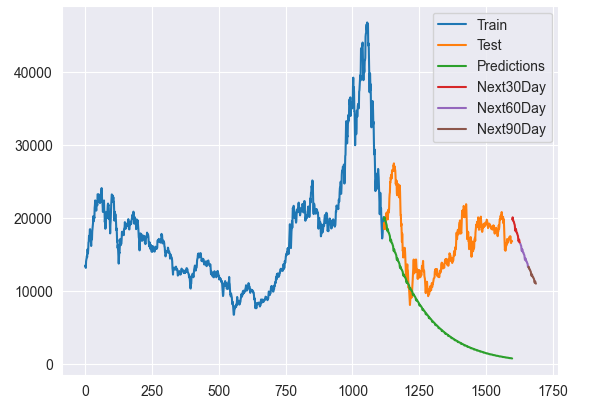
\includegraphics[width=1\textwidth]{experiment/ets/TEAM4_ETS_DIG_7_3.png}
    \caption{ETS DIG 7-3}
    \label{fig:nvl_boxplot}
    \end{minipage}
    \hfill
    \begin{minipage}{0.23\textwidth}
    \centering
    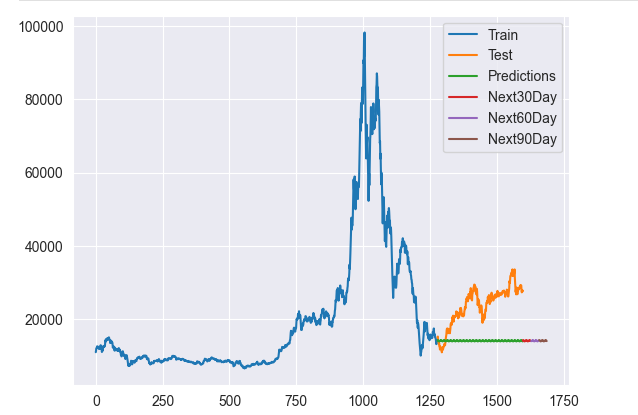
\includegraphics[width=1\textwidth]{experiment/ets/TEAM4_ETS_DIG_8_2.png}
    \caption{ETS DIG 8-2}
    \label{fig:nvl_histogram}
    \end{minipage}
    \begin{minipage}{0.23\textwidth}
    \centering
    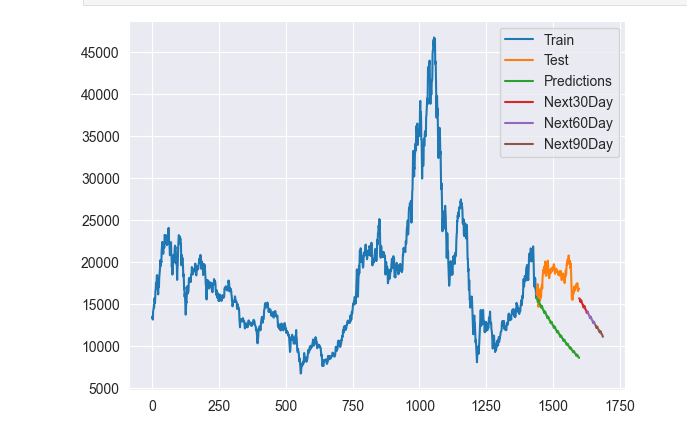
\includegraphics[width=1\textwidth]{experiment/ets/TEAM4_ETS_DIG_9_1.png}
    \caption{ETS DIG 9-1}
    \label{fig:nvl_histogram}
    \end{minipage}

    \vspace{0.5cm} % Add vertical space between the sets of figures

    \begin{minipage}{0.23\textwidth}
    \centering
    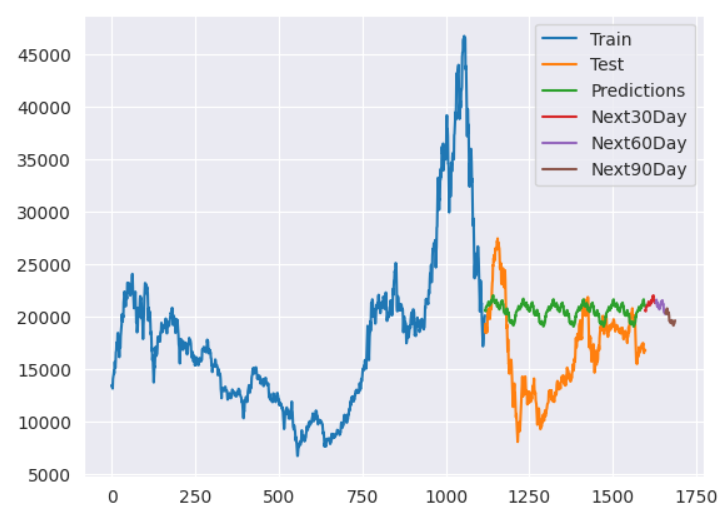
\includegraphics[width=1\textwidth]{experiment/ets/TEAM4_ETS_DXG_7_3.png}
    \caption{ETS DXG 7-3}
    \label{fig:nvl_boxplot}
    \end{minipage}
    \hfill
    \begin{minipage}{0.23\textwidth}
    \centering
    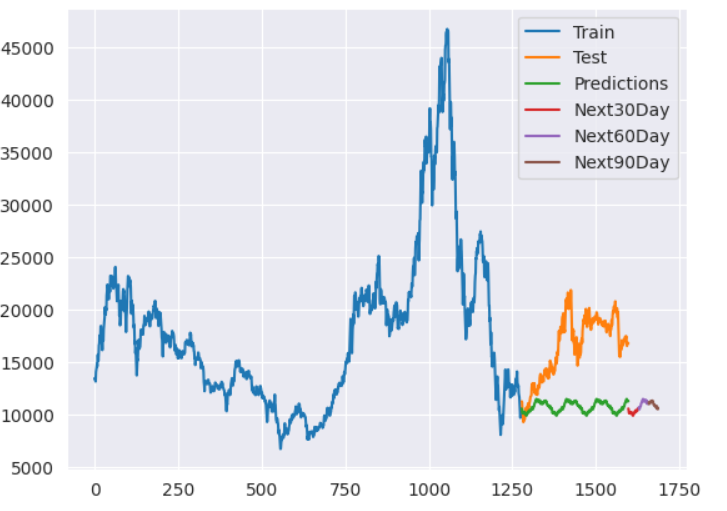
\includegraphics[width=1\textwidth]{experiment/ets/TEAM4_ETS_DXG_8_2.png}
    \caption{ETS DXG 8-2}
    \label{fig:nvl_histogram}
    \end{minipage}
    \begin{minipage}{0.23\textwidth}
    \centering
    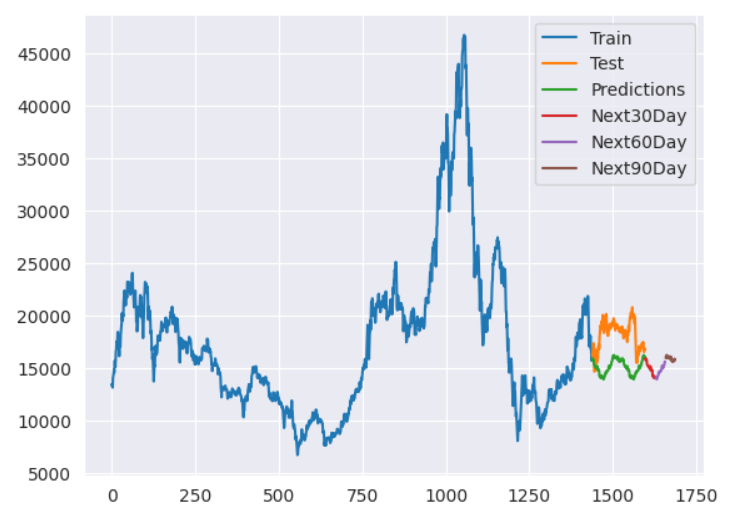
\includegraphics[width=1\textwidth]{experiment/ets/TEAM4_ETS_DXG_9_1.png}
    \caption{ETS DXG 9-1}
    \label{fig:nvl_histogram}
    \end{minipage}

    \begin{minipage}{0.23\textwidth}
    \centering
    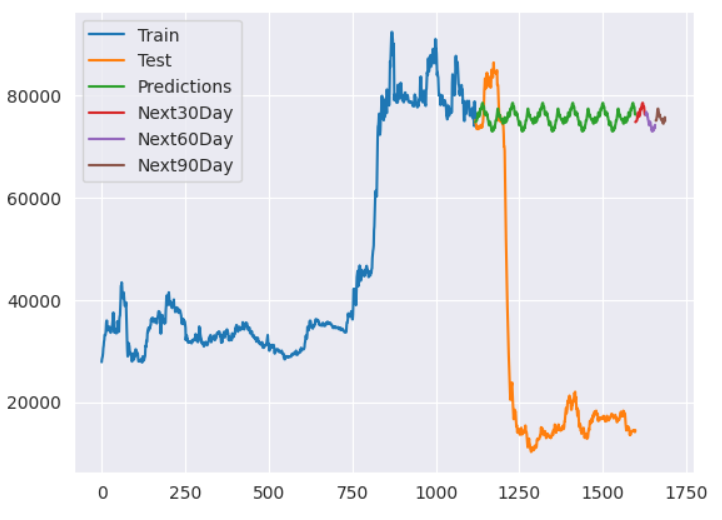
\includegraphics[width=1\textwidth]{experiment/ets/TEAM4_ETS_NVL_7_3.png}
    \caption{ETS NVL 7-3}
    \label{fig:nvl_boxplot}
    \end{minipage}
    \hfill
    \begin{minipage}{0.23\textwidth}
    \centering
    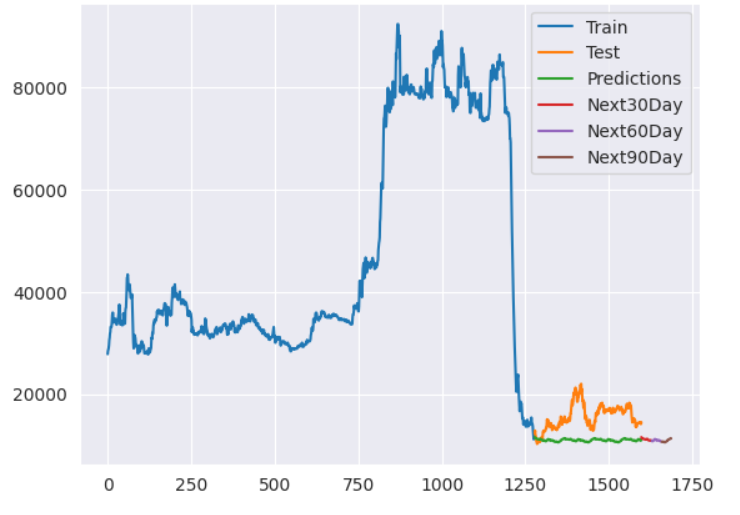
\includegraphics[width=1\textwidth]{experiment/ets/TEAM4_ETS_NVL_8_2.png}
    \caption{ETS NVL 8-2}
    \label{fig:nvl_histogram}
    \end{minipage}
    \begin{minipage}{0.23\textwidth}
    \centering
    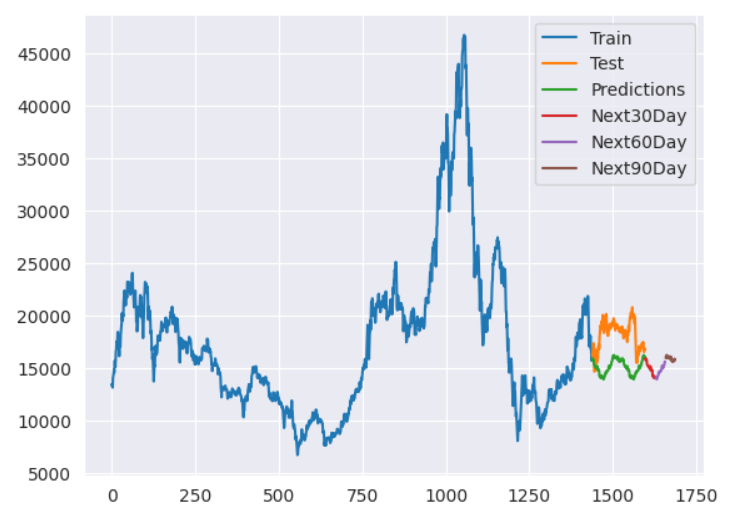
\includegraphics[width=1\textwidth]{experiment/ets/TEAM4_ETS_DXG_9_1.png}
    \caption{ETS NVL 9-1}
    \label{fig:nvl_histogram}
    \end{minipage}
\end{figure}


\begin{figure}[htbp]
\subsection{Kalman Filter}
\centering
    \begin{minipage}{0.23\textwidth}
    \centering
    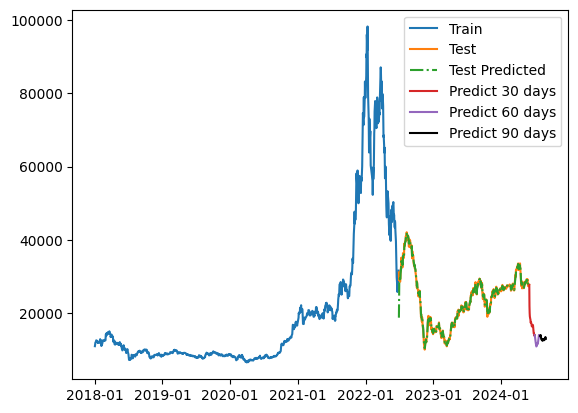
\includegraphics[width=1\textwidth]{experiment/kf/DIG 7-3.png}
    \caption{Kalman Filter DIG 7-3}
    \label{fig:nvl_boxplot}
    \end{minipage}
    \hfill
    \begin{minipage}{0.23\textwidth}
    \centering
    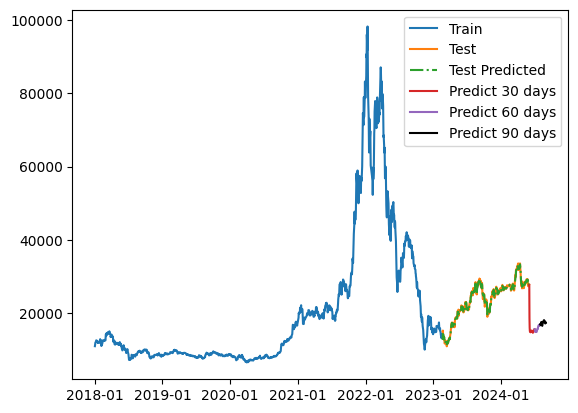
\includegraphics[width=1\textwidth]{experiment/kf/dig 8-2.png}
    \caption{Kalman Filter DIG 8-2}
    \label{fig:nvl_histogram}
    \end{minipage}
    \begin{minipage}{0.23\textwidth}
    \centering
    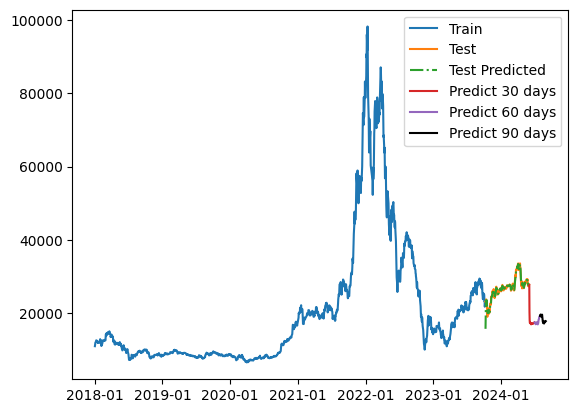
\includegraphics[width=1\textwidth]{experiment/kf/DIG 9-1.png}
    \caption{Kalman Filter DIG 9-1}
    \label{fig:nvl_histogram}
    \end{minipage}

    \vspace{0.5cm} % Add vertical space between the sets of figures

    \begin{minipage}{0.23\textwidth}
    \centering
    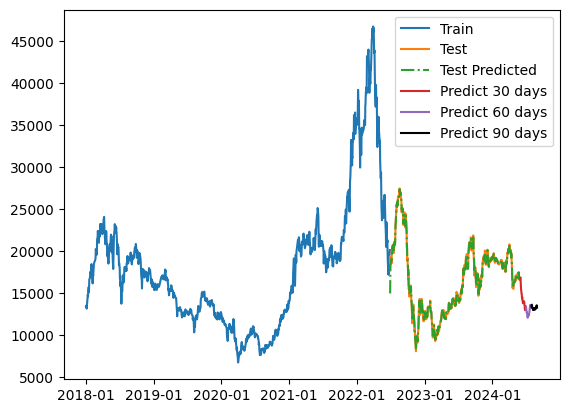
\includegraphics[width=1\textwidth]{experiment/kf/DXG 7-3.png}
    \caption{Kalman Filter DXG 7-3}
    \label{fig:nvl_boxplot}
    \end{minipage}
    \hfill
    \begin{minipage}{0.23\textwidth}
    \centering
    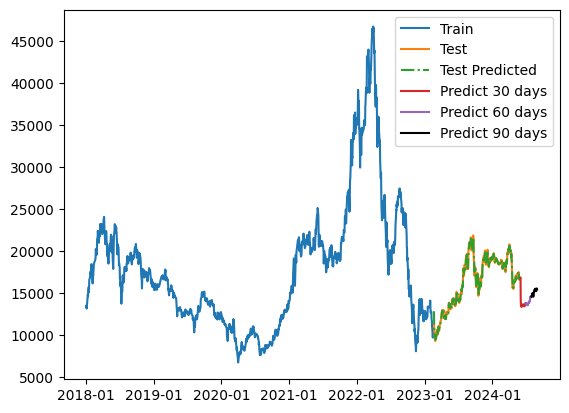
\includegraphics[width=1\textwidth]{experiment/kf/DXG 8-2.png}
    \caption{Kalman Filter DXG 8-2}
    \label{fig:nvl_histogram}
    \end{minipage}
    \begin{minipage}{0.23\textwidth}
    \centering
    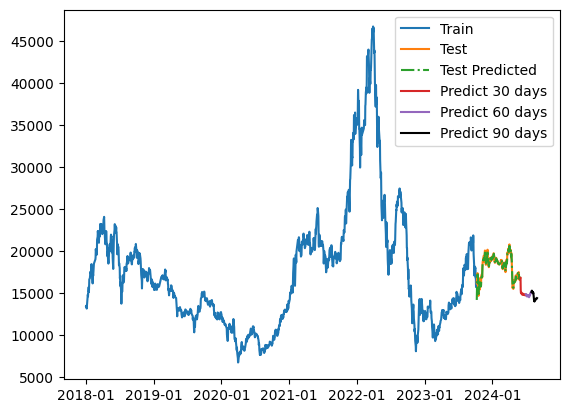
\includegraphics[width=1\textwidth]{experiment/kf/DXG 9-1.png}
    \caption{Kalman Filter DXG 9-1}
    \label{fig:nvl_histogram}
    \end{minipage}

    \begin{minipage}{0.23\textwidth}
    \centering
    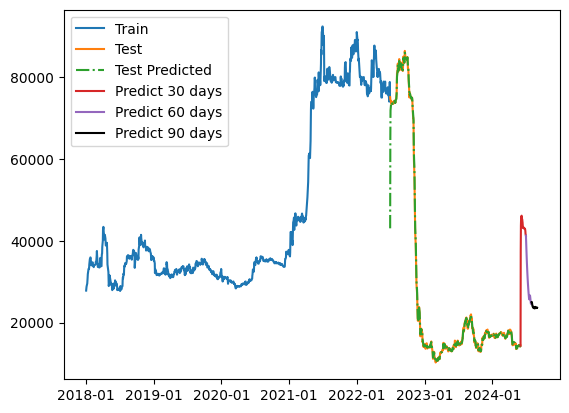
\includegraphics[width=1\textwidth]{experiment/kf/NVL 7-3.png}
    \caption{Kalman Filter NVL 7-3}
    \label{fig:nvl_boxplot}
    \end{minipage}
    \hfill
    \begin{minipage}{0.23\textwidth}
    \centering
    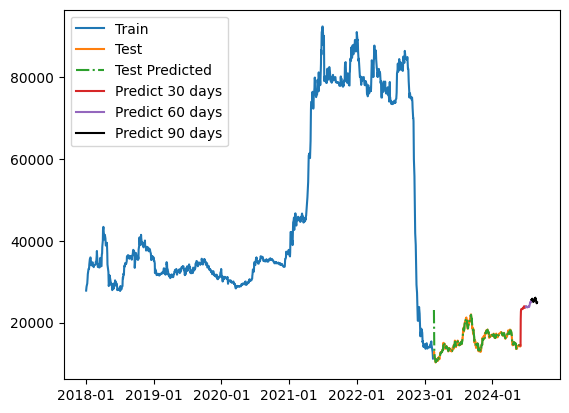
\includegraphics[width=1\textwidth]{experiment/kf/NVL 8-2.png}
    \caption{Kalman Filter NVL 8-2}
    \label{fig:nvl_histogram}
    \end{minipage}
    \begin{minipage}{0.23\textwidth}
    \centering
    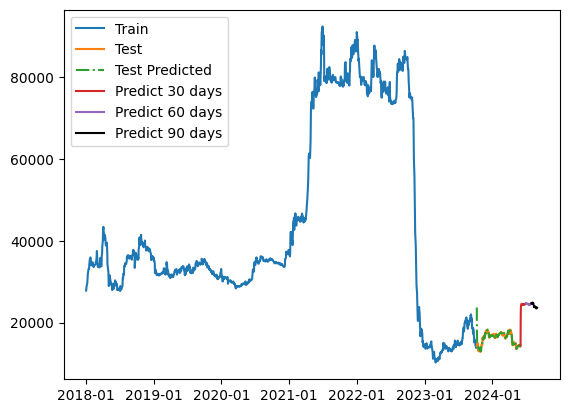
\includegraphics[width=1\textwidth]{experiment/kf/NVL 9-1.png}
    \caption{Kalman Filter NVL 9-1}
    \label{fig:nvl_histogram}
    \end{minipage}
\end{figure}

\pagebreak
\begin{figure}[htbp]
\subsection{Resnet}
\centering
    \begin{minipage}{0.23\textwidth}
    \centering
    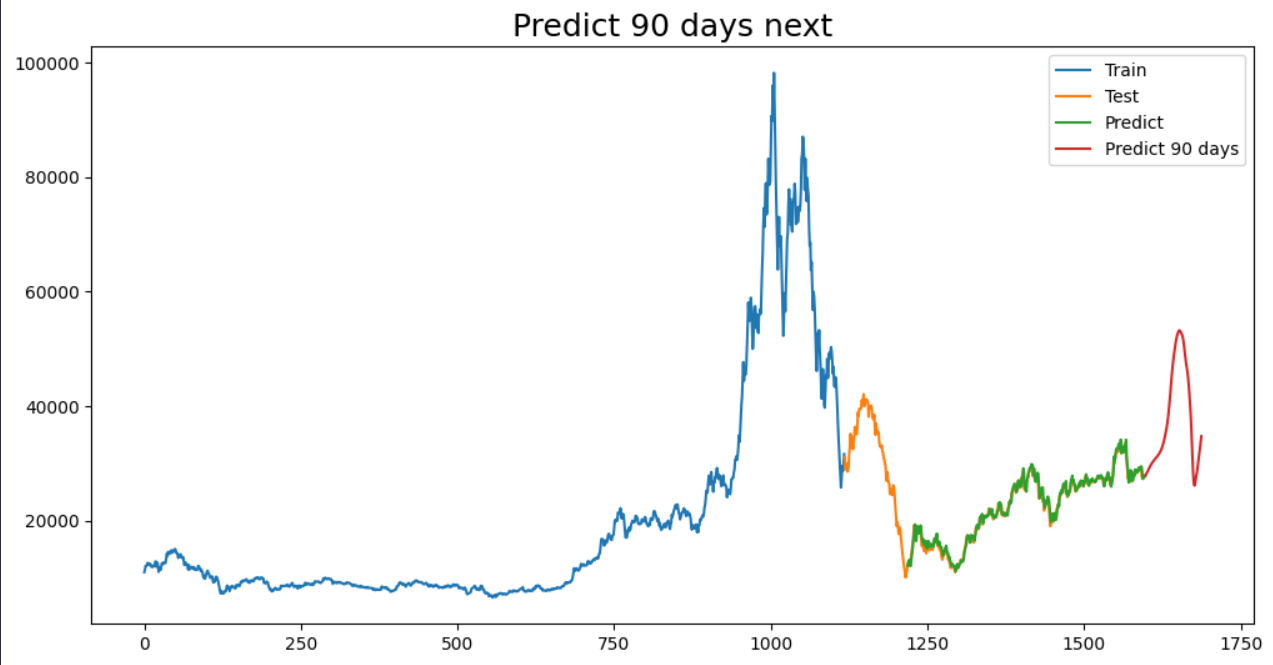
\includegraphics[width=1\textwidth]{experiment/resnet/DIG 7_3.png}
    \caption{ResNet DIG 7-3}
    \label{fig:nvl_boxplot}
    \end{minipage}
    \hfill
    \begin{minipage}{0.23\textwidth}
    \centering
    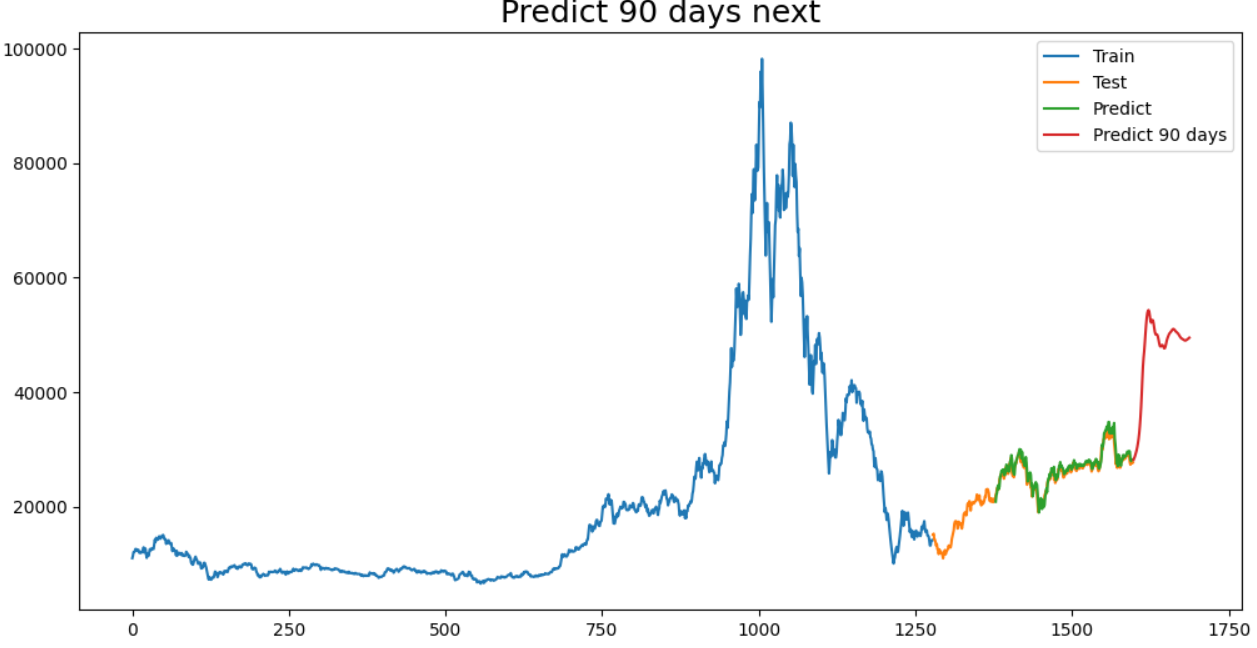
\includegraphics[width=1\textwidth]{experiment/resnet/DIG 8_2.png}
    \caption{ResNet DIG 8-2}
    \label{fig:nvl_histogram}
    \end{minipage}
    \begin{minipage}{0.23\textwidth}
    \centering
    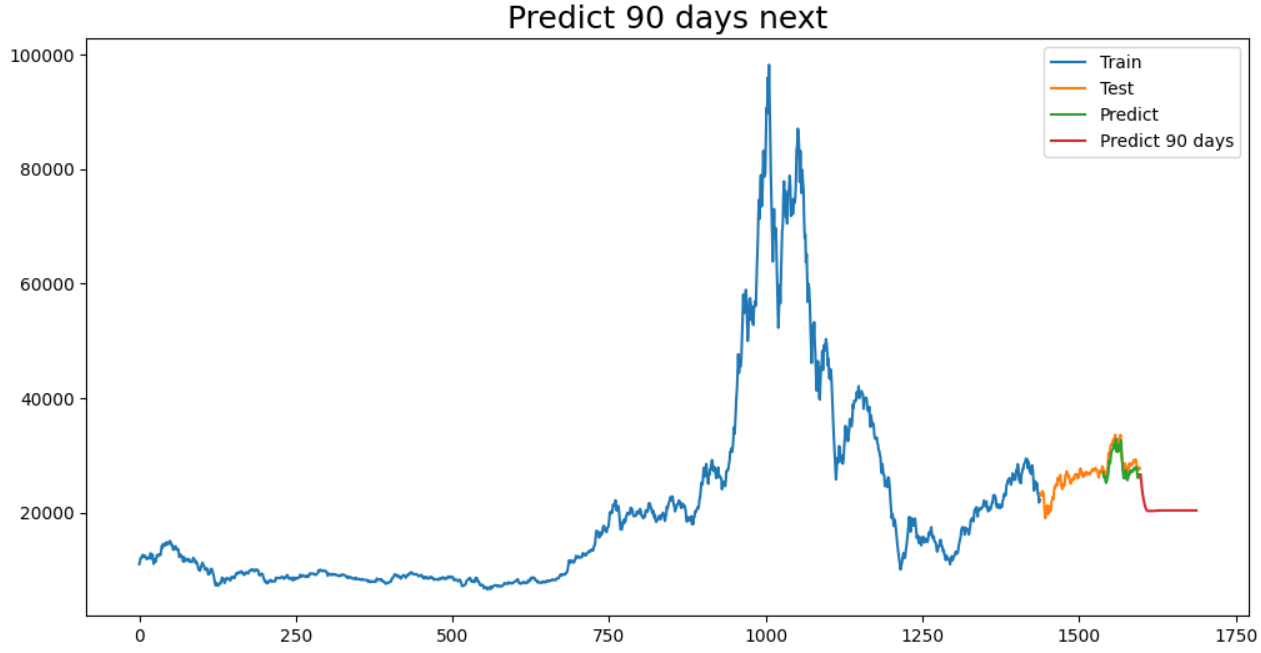
\includegraphics[width=1\textwidth]{experiment/resnet/DIG 9_1.png}
    \caption{ResNet DIG 9-1}
    \label{fig:nvl_histogram}
    \end{minipage}

    \vspace{0.5cm} % Add vertical space between the sets of figures

    \begin{minipage}{0.23\textwidth}
    \centering
    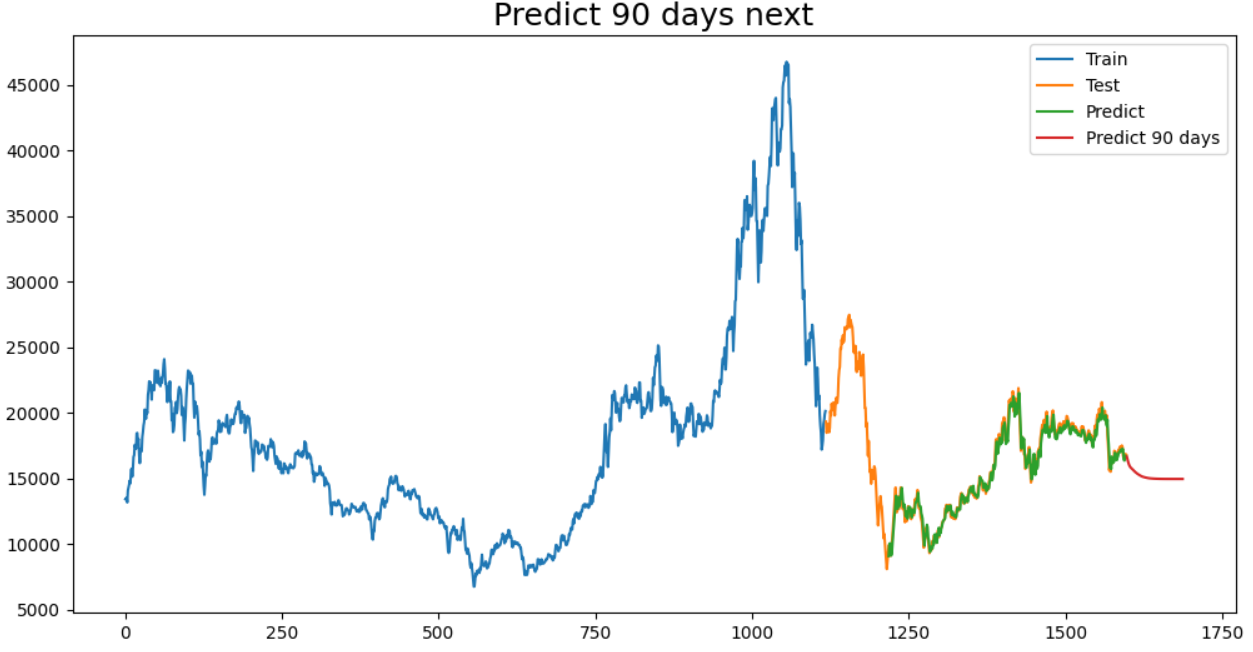
\includegraphics[width=1\textwidth]{experiment/resnet/DXG 7_3.png}
    \caption{ResNet DXG 7-3}
    \label{fig:nvl_boxplot}
    \end{minipage}
    \hfill
    \begin{minipage}{0.23\textwidth}
    \centering
    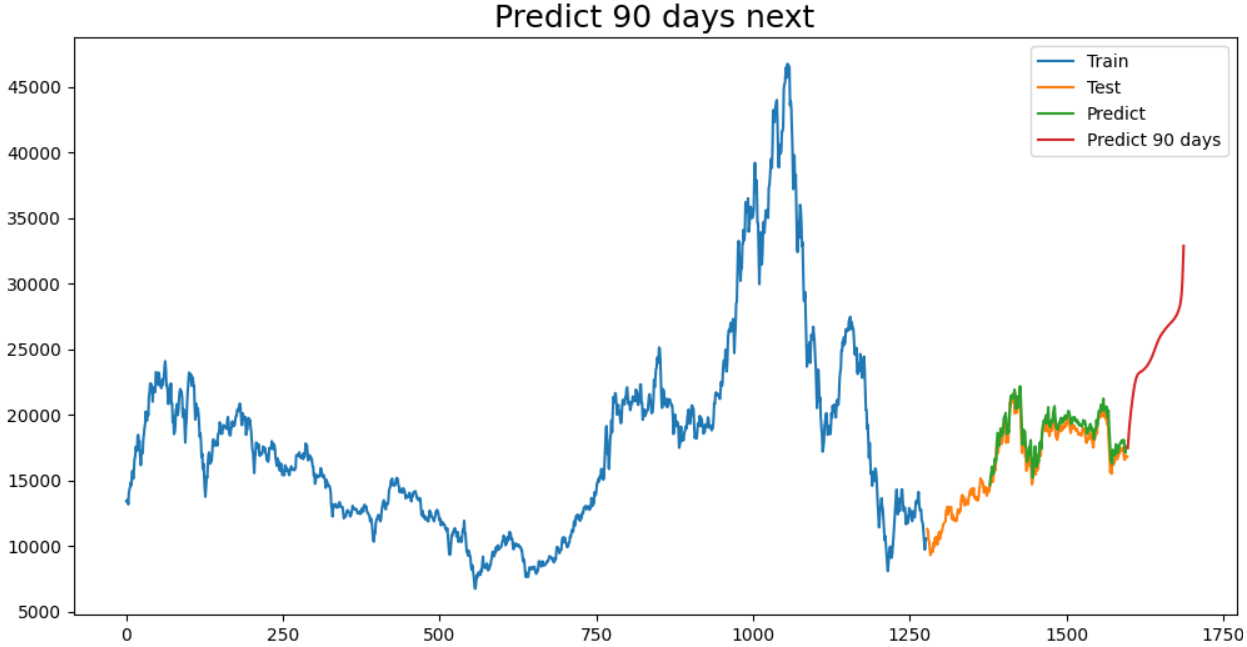
\includegraphics[width=1\textwidth]{experiment/resnet/DXG 8_2.png}
    \caption{ResNet DXG 8-2}
    \label{fig:nvl_histogram}
    \end{minipage}
    \begin{minipage}{0.23\textwidth}
    \centering
    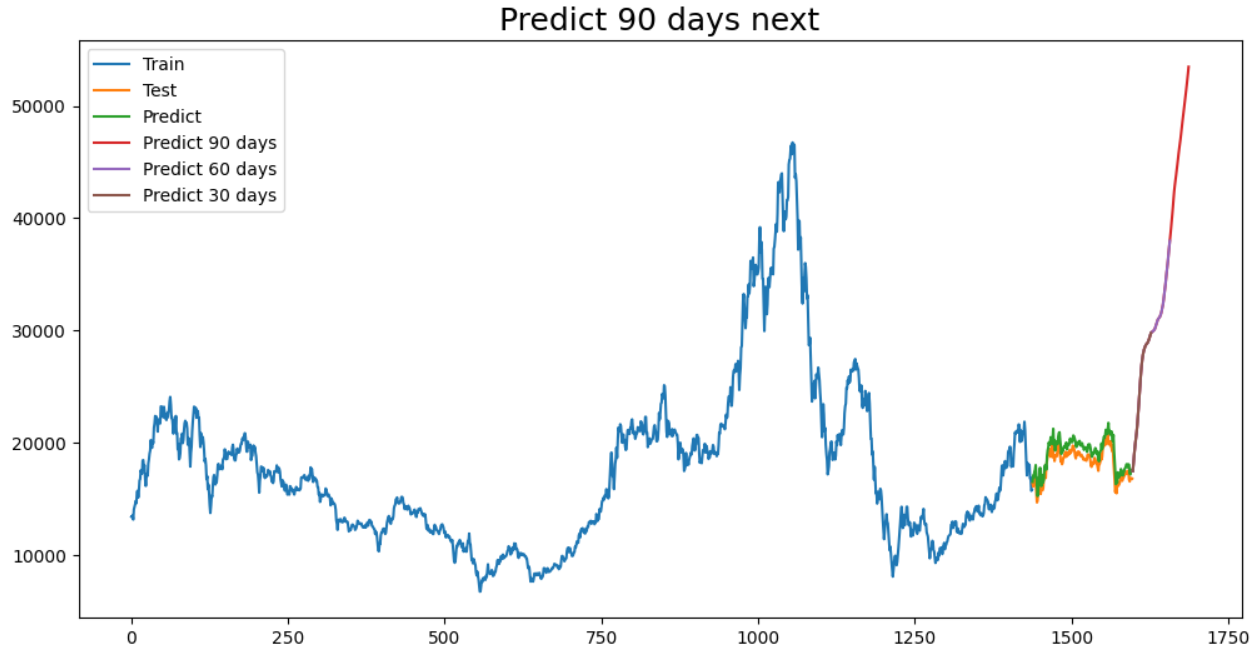
\includegraphics[width=1\textwidth]{experiment/resnet/DXG 9_1.png}
    \caption{ResNet DXG 9-1}
    \label{fig:nvl_histogram}
    \end{minipage}

    \begin{minipage}{0.23\textwidth}
    \centering
    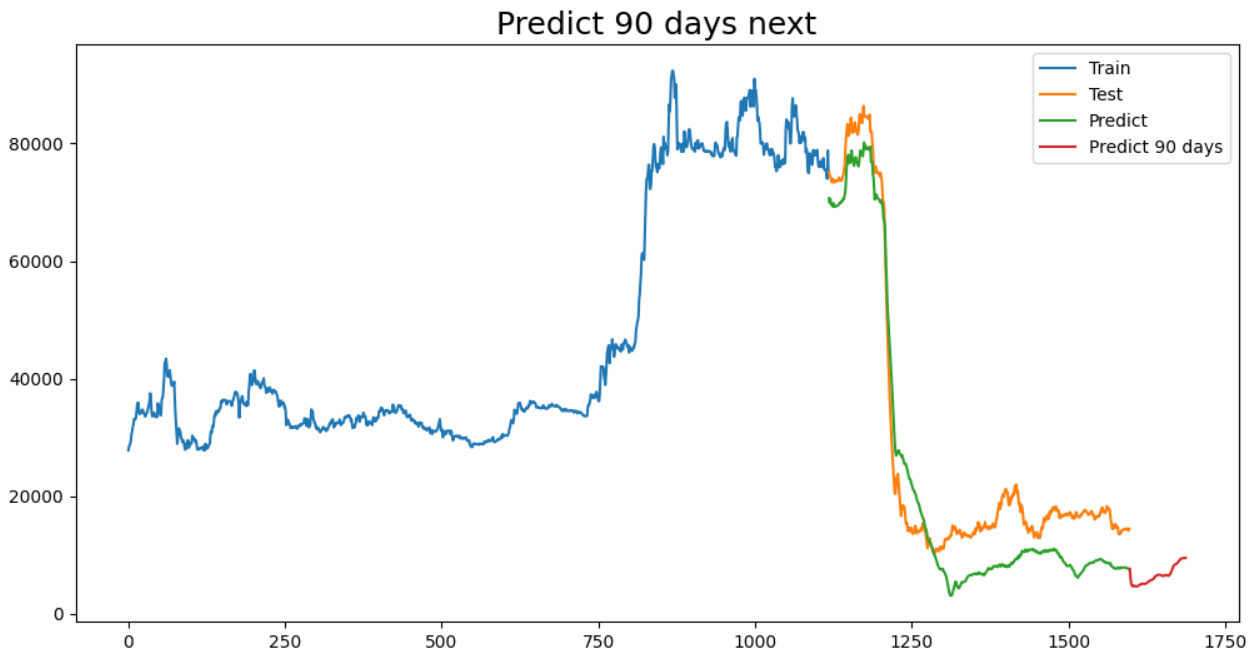
\includegraphics[width=1\textwidth]{experiment/resnet/NVL 7_3.png}
    \caption{ResNet NVL 7-3}
    \label{fig:nvl_boxplot}
    \end{minipage}
    \hfill
    \begin{minipage}{0.23\textwidth}
    \centering
    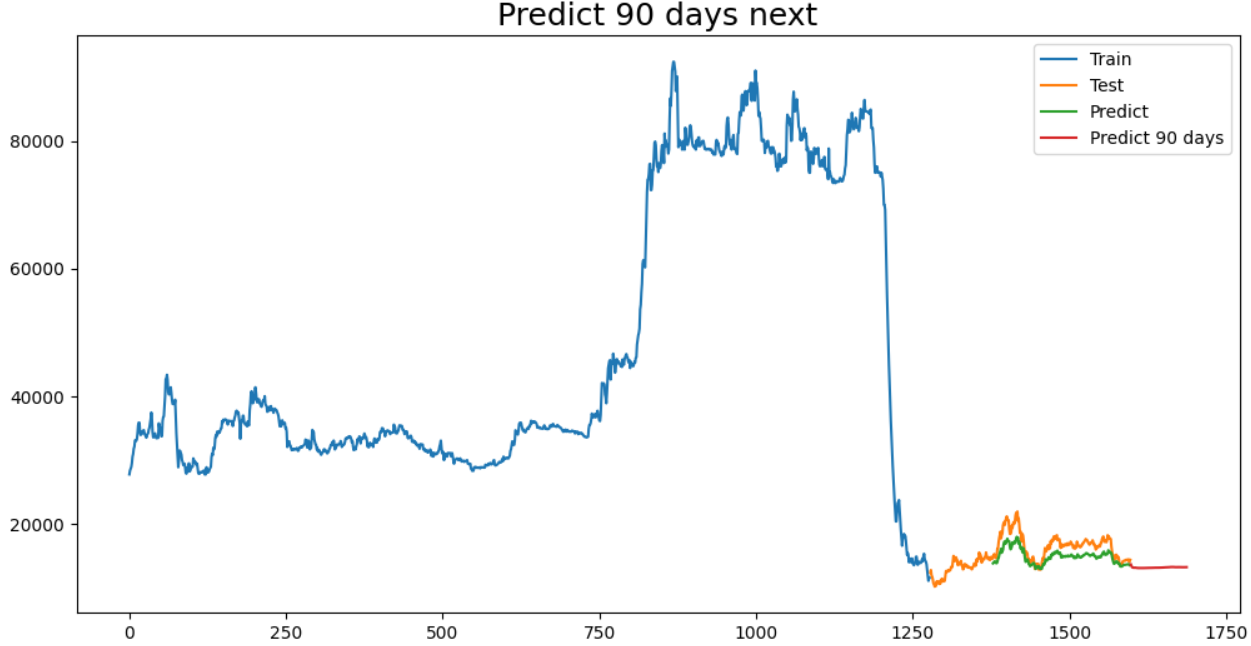
\includegraphics[width=1\textwidth]{experiment/resnet/NVL 8_2.png}
    \caption{ResNet NVL 8-2}
    \label{fig:nvl_histogram}
    \end{minipage}
    \begin{minipage}{0.23\textwidth}
    \centering
    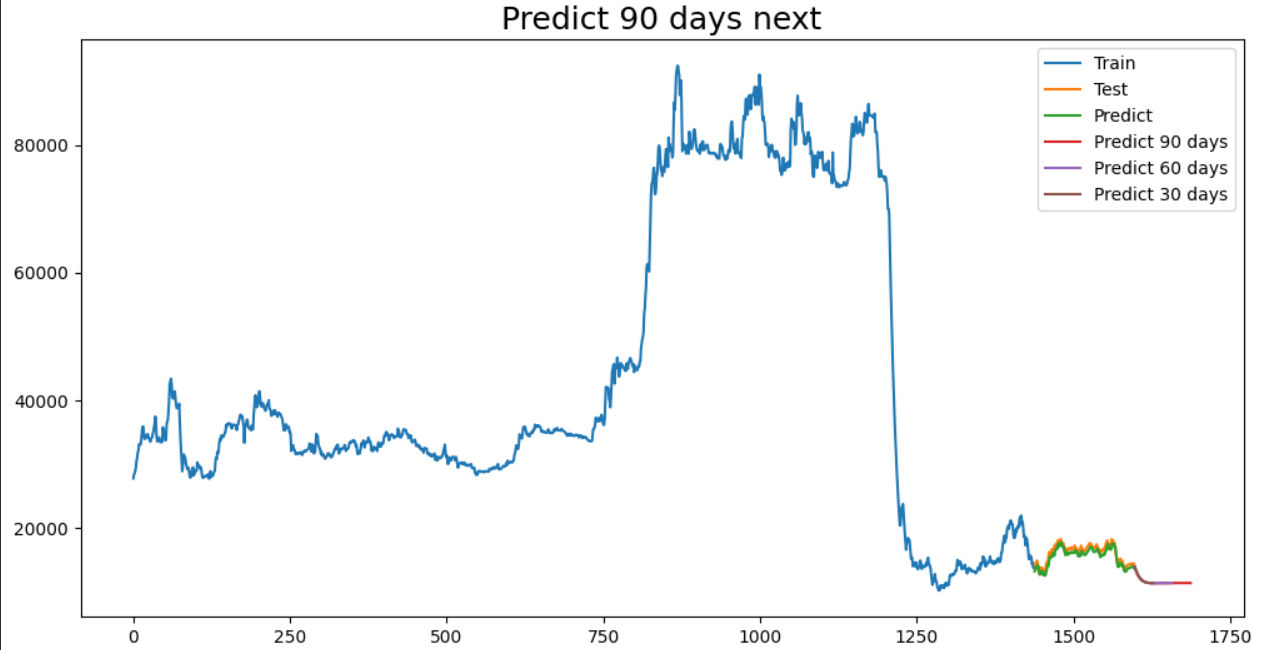
\includegraphics[width=1\textwidth]{experiment/resnet/NVL 9_1.png}
    \caption{ResNet NVL 9-1}
    \label{fig:nvl_histogram}
    \end{minipage}
\end{figure}



% \subsection{Model Evaluation with NVL Dataset}



\section{Evaluation}
\begin{table*}
    \centering
    \caption{Models evaluation}
    \label{tb_evaluation}
    \begin{adjustbox}{center=\textwidth}
    \begin{tabular}{|c|c|c|c|c|c|c|c|c|c|c|}
        \hline
        \multirow{2}{*}{\textbf{Model}} & \multirow{2}{*}{\textbf{Ratio}} & \multicolumn{3}{c|}{\textbf{NVL dataset}} & \multicolumn{3}{c|}{\textbf{DIG dataset}} & \multicolumn{3}{c|}{\textbf{DXG dataset}} \\ \cline{3-11}
        & & \textbf{MAE} & \textbf{MAPE (\%)} & \textbf{RMSE} & \textbf{MAE} & \textbf{MAPE (\%)} & \textbf{RMSE} & \textbf{MAE} & \textbf{MAPE (\%)} & \textbf{RMSE}\\ \hline
        \multirow{3}{*}{\textbf{\makecell{ETS}}} 
            & 7:3 & 48998.495 & 314.2 & 53609.076 & 9797.853 & 53.264 & 11402.122 & 4640.983&34.413	&5605.060 \\ 
            & 8:2 & 4661.080 & 28.220 & 5224.060 & 9903.334 & 38.465 & 11037.222 & 5769.899	& 32.560& 	6481.276 \\ 
            & 9:1 & 2366.397 & 14.043 & 2366.397 & 6144.315 &	21.926& 6885.692 & 3081.405	& 16.460 &	3459.589 \\ \hline
        \multirow{3}{*}{\textbf{TBATS}} 
            & 7:3 & 47834.068 &	307 &	52333.638 & 9343.219	&511 &	10964.319 & 3866.195 &	286 &	4856.482 \\
            & 8:2 & 5735.103 & 35.1 &	6267.973 & 9896.617 &	38.8 &	10921.963	&	6577.959 &	36.07 &	7251.366 \\
            & 9:1 & 4402.614 &	26.6 &	4732.264 & 5224.725	& 18.6&	5841.843&	2968.839&	15.9 &	3259.942 \\ \hline
        \multirow{3}{*}{\textbf{Kalman Filter}} 
            & 7:3 & 248.394&	0.857&	1555.819&	250.028&	0.114&	656.425&	128.101&	0.816 &	257.248 \\
            & 8:2 & 139.208&	0.827&	635.127&	189.296 &	0.863&	281.185&	102.684&	0.645&	161.435 \\
            & 9:1 & 157.4223 & 0.8653 & 781.5291 & 814.8535 & 1.0641 & 670.1075 & 109.9869 & 0.6388 & 218.9151 \\ \hline
        \multirow{3}{*}{\textbf{ResNET}} 
            & 7:3 & 6680.6057 & 36.78 & 7215.2 & 7215.2 & 21.33 & 5276.83 & 890.51 & 5.76 & 1252.69 \\
            & 8:2 & 5097.91 & 33.48 & 6181.73 & 6181.73 & 9.53 & 2610.58 & 632.27 & 4.32 & 778.4 \\
            & 9:1 & 6162.79 & 39.18 & 6351.53 & 2298.18 & 8.26 & 2623.84 & 2623.84 & 4.77 & 967.51 \\ \hline
        \multirow{3}{*}{\textbf{FEDFormer}} 
            & 7:3 & 65368.2816 & 414.384 & 70851.3612 & 107217.0713 & 466.525 & 120589.3802 & 16015.6167 & 104.243 & 18241.8151 \\
            & 8:2 & 11452.2032 & 77.522 & 11732.3351 & 6986.1019 & 27.896 & 7780.4389 & 5084.8468 & 28.707 & 6174.6696 \\
            & 9:1 & 1167.8452 & 7.365 & 1352.7104 & 4040.3271 & 14.522 & 4490.0098 & 8672.5042 & 47.231 & 8880.7576 \\ \hline
    \end{tabular}
    \end{adjustbox}
\end{table*}


% \begin{table}[htbp]

% \subsection{Model Evaluation with NVL Dataset}
% \caption{7-3 Train-Test Ratio}
% \begin{center}
% \begin{tabular}{|c|c|c|c|}
% \hline
% \textbf{Evaluation}&\multicolumn{3}{|c|}{\textbf{Evaluation Metric}} \\
% \cline{2-4} 
% \textbf{Model} & \textbf{\textit{MAE}}& \textbf{\textit{MAPE}}& \textbf{\textit{RMSE}} \\
% \hline
% ETS & 48998.495 & 3.142 & 53609.076\\
% \hline
% TBATS & 47834.068 & 3.070 & 52333.638\\
% \hline
% Kalman Filter & 248.394 & 0.857 & 1555.819\\
% \hline
% ResNet & 6680.6057 & 36.78 & 7215.2\\
% \hline
% ResNetLSTM & 26855.33 & 183.2 & 31783.7\\
% \hline
% Fedformer & 26855.33 & 183.2 & 31783.7\\
% \hline
% \end{tabular}
% \label{tab1}
% \end{center}
% \end{table}

% \begin{table}[htbp]
% \caption{8-2 Train-Test Ratio}
% \begin{center}
% \begin{tabular}{|c|c|c|c|}
% \hline
% \textbf{Evaluation}&\multicolumn{3}{|c|}{\textbf{Evaluation Metric}} \\
% \cline{2-4} 
% \textbf{Model} & \textbf{\textit{MAE}}& \textbf{\textit{MAPE}}& \textbf{\textit{RMSE}} \\
% \hline
% ETS & 4661.080 & 0.282 & 5224.061\\
% \hline
% TBATS & 5735.103 & 0.351 & 6267.973\\
% \hline
% Kalman Filter & 139.208 & 0.827 & 635.127\\
% \hline
% ResNet & 1692.589 & 9.690 & 1916.366\\
% \hline
% \end{tabular}
% \label{tab1}
% \end{center}
% \end{table}

% \begin{table}[htbp]
% \caption{9-1 Train-Test Ratio}
% \begin{center}
% \begin{tabular}{|c|c|c|c|}
% \hline
% \textbf{Evaluation}&\multicolumn{3}{|c|}{\textbf{Evaluation Metric}} \\
% \cline{2-4} 
% \textbf{Model} & \textbf{\textit{MAE}}& \textbf{\textit{MAPE}}& \textbf{\textit{RMSE}} \\
% \hline
% ETS & 2366.397 & 0.140 & 2741.858\\
% \hline

% TBATS & 4402,614 & 0,266 & 4732,264\\
% \hline
% Kalman Filter & 157.422 & 0.865 & 781.529\\
% \hline
% ResNet & 477.017 & 3.018 & 551.227\\
% \hline
% \end{tabular}
% \label{tab1}
% \end{center}
% \end{table}

% % \subsection{Model Evaluation with DIG Dataset}

% \begin{table}[htbp]
% \subsection{Model Evaluation with DIG Dataset}
% \caption{7-3 Train-Test Ratio}
% \begin{center}
% \begin{tabular}{|c|c|c|c|}
% \hline
% \textbf{Evaluation}&\multicolumn{3}{|c|}{\textbf{Evaluation Metric}} \\
% \cline{2-4} 
% \textbf{Model} & \textbf{\textit{MAE}}& \textbf{\textit{MAPE}}& \textbf{\textit{RMSE}} \\
% \hline
% ETS & 9797.853 & 0.533 & 11402.122\\
% \hline
% TBATS & 9343.220 & 0.5107 & 10964.319\\
% \hline
% Kalman Filter & 250.028 & 1.144 & 656,425\\
% \hline
% ResNet & 608.818 & 2.916 & 784.812\\
% \hline
% \end{tabular}
% \label{tab1}
% \end{center}
% \end{table}

% \begin{table}[htbp]
% \caption{8-2 Train-Test Ratio}
% \begin{center}
% \begin{tabular}{|c|c|c|c|}
% \hline
% \textbf{Evaluation}&\multicolumn{3}{|c|}{\textbf{Evaluation Metric}} \\
% \cline{2-4} 
% \textbf{Model} & \textbf{\textit{MAE}}& \textbf{\textit{MAPE}}& \textbf{\textit{RMSE}} \\
% \hline
% ETS & 9903.334 & 0.385 & 11037.223\\
% \hline
% TBATS & 9896.617 & 0.388 & 10921.963\\
% \hline
% Kalman Filter & 189.296 & 0.863 & 281.185\\
% \hline
% ResNet & 721.758 & 2.758 & 937.697\\
% \hline
% \end{tabular}
% \label{tab1}
% \end{center}
% \end{table}

% \begin{table}[htbp]
% \caption{9-1 Train-Test Ratio}
% \begin{center}
% \begin{tabular}{|c|c|c|c|}
% \hline
% \textbf{Evaluation}&\multicolumn{3}{|c|}{\textbf{Evaluation Metric}} \\
% \cline{2-4} 
% \textbf{Model} & \textbf{\textit{MAE}}& \textbf{\textit{MAPE}}& \textbf{\textit{RMSE}} \\
% \hline
% ETS & 6144.316 & 0.219 & 6885.692\\
% \hline
% TBATS & 5224.725 & 0.186 & 5841.843\\
% \hline
% Kalman Filter & 243.186 & 1.064 & 670.108\\
% \hline
% ResNet & 1241.867 & 4.187 & 1407.779\\
% \hline
% \end{tabular}
% \label{tab1}
% \end{center}
% \end{table}


% \begin{table}[htbp]
% \subsection{Model Evaluation with DXG Dataset}
% \caption{7-3 Train-Test Ratio}
% \begin{center}
% \begin{tabular}{|c|c|c|c|}
% \hline
% \textbf{Evaluation}&\multicolumn{3}{|c|}{\textbf{Evaluation Metric}} \\
% \cline{2-4} 
% \textbf{Model} & \textbf{\textit{MAE}}& \textbf{\textit{MAPE}}& \textbf{\textit{RMSE}} \\
% \hline
% ETS & 12978.866 & 0.8054 & 13836.799\\
% \hline
% TBATS & 3866.195 & 0.286 & 4856.482\\
% \hline
% Kalman Filter & 128.100 & 0.816 & 257.248\\
% \hline
% ResNet & 727.179 & 4.903 & 887.615\\
% \hline
% \end{tabular}
% \label{tab1}
% \end{center}
% \end{table}

% \begin{table}[htbp]
% \caption{8-2 Train-Test Ratio}
% \begin{center}
% \begin{tabular}{|c|c|c|c|}
% \hline
% \textbf{Evaluation}&\multicolumn{3}{|c|}{\textbf{Evaluation Metric}} \\
% \cline{2-4} 
% \textbf{Model} & \textbf{\textit{MAE}}& \textbf{\textit{MAPE}}& \textbf{\textit{RMSE}} \\
% \hline
% ETS & 5769.899 & 0.326 & 6481.277\\
% \hline
% TBATS & 6577.959 & 0.374 & 7251.366\\
% \hline
% Kalman Filter & 102.684 & 0.645 & 161.435\\
% \hline
% ResNet & 653.404 & 3.647 & 777.722\\
% \hline
% \end{tabular}
% \label{tab1}
% \end{center}
% \end{table}

% \begin{table}[htbp]
% \caption{9-1 Train-Test Ratio}
% \begin{center}
% \begin{tabular}{|c|c|c|c|}
% \hline
% \textbf{Evaluation}&\multicolumn{3}{|c|}{\textbf{Evaluation Metric}} \\
% \cline{2-4} 
% \textbf{Model} & \textbf{\textit{MAE}}& \textbf{\textit{MAPE}}& \textbf{\textit{RMSE}} \\
% \hline
% TBATS & 2968.839 & 0.159 & 3259.942\\
% \hline
% Kalman Filter & 109,987 & 0,639 & 218.915\\
% \hline
% ResNet & 462.808 & 2.582 & 557.948\\
% \hline
% \end{tabular}
% \label{tab1}
% \end{center}
% \end{table}

\newpage
\section{Conclusion}
Five machine learning and deep learning algorithms—FEDformer, TBATS, ETS, Kalman Filter, and ResNet—were found useful in predicting stock values for three major Vietnamese real estates. Our comprehensive research revealed that each algorithm has its own strengths and drawbacks; ResNet are particularly good at capturing complex patterns while Kalman Filter and TBATS work better with simple trends. ETS and FEDformer is a method of balanced type which gives modest computational requirements but still provides reasonable accuracy.

To sum up, the correct algorithm will depend on the characteristics of the time-series data as well as forecasting requirements. This study provides valuable insights and practical recommendations on selection and implementation of these algorithms within the context of real estate industry. In future studies it would be interesting to examine more diversified datasets taking into account other such factors as economic indicators in order to improve predictive accuracy and applicability to various practical situations.
\section*{Acknowledgment}

We thank Assoc. Prof. Dr. Nguyen Dinh Thuan and Mr. Nguyen Minh Nhut for their invaluable support and guidance throughout our research.



\begin{thebibliography}{00}
\bibitem{b1}A. T. Haryono, R. Sarno and K. R. Sungkono, "Transformer-Gated Recurrent Unit Method for Predicting Stock Price Based on News Sentiments and Technical Indicators," IEEE Journals \& Magazine | IEEE Xplore, 2023, 
\bibitem{b2}H. Liu and B. Song, "Stock Price Trend Prediction Model Based on Deep Residual Network and Stock Price Graph," IEEE Conference Publication | IEEE Xplore, Dec. 01, 2018. 
\bibitem{b3}S. Khan and H. Alghulaiakh, “ARIMA model for accurate Time series stocks Forecasting,” International Journal of Advanced Computer Science and Applications/International Journal of Advanced Computer Science \& Applications, vol. 11, no. 7, Jan. 2020, doi: 10.14569/ijacsa.2020.0110765.
\bibitem{b4}Zhuge Q, Xu L, Zhang G (2017) "LSTM neural network with emotional analysis for prediction of stock price," Eng Lett 2(25):167–175. http://www.engineeringletters.com/issues\_v25/issue\_2/EL\_25\_2\_09.pdf
\bibitem{b5}Selvin, S., Vinayakumar, R., Gopalakrishnan, E. A., Menon, V. K., \& Soman, K. P, “Stock price prediction using LSTM, RNN and CNN-sliding window model,” IEEE Conference Publication | IEEE Xplore, Sep. 01, 2017. 
\bibitem{b6}C. Qi, J. Ren, and J. Su, “GRU Neural Network based on CEEMDAN–Wavelet for stock price prediction”, Applied Sciences, vol. 13, no. 12, p. 7104, Jun. 2023, doi: 10.3390/app13127104.
\bibitem{b7}Z. Sun, “Comparison of Trend Forecast Using ARIMA and ETS Models for S\&P500 Close Price,” ACM Journal, Oct. 2020, doi: 10.1145/3436209.3436894. 
doi:10.1145/3436209.3436894
\bibitem{b8}R. Seethalakshmi, “Analysis of stock market predictor variables using Linear Regression” International Journal of Pure and Applied Mathematics, vol. 119, no. 15, p. 369-378, Jan. 2018
\bibitem{b9} I. Sadia, A. Mahmood; L. B. M. Kiah, S. R. Azzuhri, "Analysis and forecasting of blockchain-based cryptocurrencies and performance evaluation of TBATS, NNAR and ARIMA.", 2022, September 13. IEEE Conference Publication | IEEE Xplore. 
\bibitem{b10} N. Deepika, M. N. Bhat,  An efficient stock market prediction method based on Kalman filter. Journal of Institution of Engineers (India) Series, 2021 B. https://doi.org/10.1007/s40031-021-00583-9

\bibitem{b11} Hanke, J. E. (2008). Business Forecasting (Vol. 8). New Jersey:
Pearson Education International.
\bibitem{b12} Hyndman, R. J., Athanasopoulos, G. (2013). Forecasting:
Principles and Practice. Melbourne: OTexts
\bibitem{b13} Rim A., GiLang R. A., Sari S. W. Time series forecasting using exponential smoothing to predict the number of website visitor of Sebelas Maret University. (2015b, October 1). IEEE Conference Publication
\bibitem{b14}Perone, G. (2021). Comparison of ARIMA, ETS, NNAR, TBATS and hybrid models to forecast the second wave of COVID-19 hospitalizations in Italy. the European Journal of Health Economics, 23(6), 917–940. https://doi.org/10.1007/s10198-021-01347-4
\bibitem{b15}Time Series classification from scratch with Deep Neural Networks: A strong baseline | IEEE conference publication | IEEE Xplore, https://ieeexplore.ieee.org/abstract/document/7966039/ (accessed Jun. 6, 2024). 
\bibitem{b16}Short-term load forecasting based on Resnet and LSTM | IEEE Conference publication | IEEE Xplore, https://ieeexplore.ieee.org/abstract/document/8587554/ (accessed Jun. 6, 2024).
\bibitem{b32}D. Zhao and H. Zhang, “The research on TBATS and ELM models for prediction of human brucellosis cases in mainland China: a time series study,” BMC infectious diseases, vol. 22, no. 1, Dec. 2022, doi: https://doi.org/10.1186/s12879-022-07919-w.
\bibitem{b20}T. Zhou, Z. Ma, Q. Wen, X. Wang, L. Sun, and R. Jin, “FEDFormer: Frequency Enhanced Decomposed Transformer for long-term series forecasting,” 2022. 
\bibitem{b21}F. Govaers, Introduction and Implementations of the Kalman Filter. BoD – Books on Demand, 2022, International Conference on Machine Learning
‌
\end{thebibliography}


\end{document}
